\documentclass[a4paper]{tufte-book}
\usepackage{lmodern}% http://ctan.org/pkg/lm
\newcounter{ccounter}
\newcounter{clatihan}
\newcounter{clisting}
\renewcommand\theccounter{\arabic{ccounter}}
\renewcommand\theclatihan{\arabic{clatihan}}
\renewcommand\theclisting{\arabic{clisting}}
\usepackage{soul,color}
\usepackage{placeins}
\usepackage{algorithmic}
\usepackage{algorithm}
\usepackage{listings}
\usepackage{lstlinebgrd}
\usepackage{graphicx}
\usepackage{makeidx}
\usepackage{mathtools}
\usepackage{bookmark}
\usepackage{xcolor}
\usepackage{mathpazo}
\usepackage{multirow}
\definecolor{codegreen}{rgb}{0,0.6,0}
\definecolor{codegray}{rgb}{0.5,0.5,0.5}
\definecolor{codepurple}{rgb}{0.58,0,0.82}
\definecolor{backcolour}{rgb}{0.95,0.95,0.92}
\definecolor{codehighlight}{rgb}{1,0.65,0.65}
 
\lstdefinestyle{pylist}{
    backgroundcolor=\color{backcolour},   
    commentstyle=\color{codegreen},
    keywordstyle=\color{magenta},
    numberstyle=\tiny\color{codegray},
    stringstyle=\color{codepurple},
    basicstyle=\footnotesize,
    breakatwhitespace=false,         
    breaklines=true,                 
    captionpos=b,                    
    keepspaces=true,                 
    numbers=left,                    
    numbersep=5pt,                  
    showspaces=false,                
    showstringspaces=false,
    showtabs=false,                  
    tabsize=2
}
 
\lstset{style=pylist}

\author{STMIK Mikroskil}
\title{Desain dan Analisis Algoritma}
\publisher{Teknik Informatika -- STMIK Mikroskil}
\newenvironment{myindentpar}[1]%
{
	\begin{list}{}%
  {
  	\setlength{\leftmargin}{#1}}%
    \item[]%
	}
{\end{list}}

\newenvironment{contoh}{
	\refstepcounter{ccounter}
	\begin{myindentpar}{1cm}
	\textbf{\underline{Contoh \arabic{ccounter}}}
}{	
	\end{myindentpar}
}

\newenvironment{latihan}{
	\refstepcounter{clatihan}
	\begin{myindentpar}{1cm}
	\textbf{\underline{Latihan \arabic{clatihan}}}	
}{	
	\end{myindentpar}
}

\newenvironment{konsep}{
	\begin{latihan}
	\small\textbf{(Konsep)}
}{
	\end{latihan}
}

\newenvironment{teori}{
    \begin{myindentpar}{1cm}
    \textbf{\underline{Teori}}
}{
    \end{myindentpar}
}

\newenvironment{pemrograman}{
	\begin{latihan}
	\small\textbf{(Pemrograman)}
}{
	\end{latihan}
}

\newenvironment{proyek}{
	\begin{latihan}
	\small\textbf{(Kelompok)}
}{
	\end{latihan}
}

\newenvironment{listprog}[1]{
	\refstepcounter{clisting}
	\begin{myindentpar}{1cm}
	\textbf{\underline{Listing \arabic{clisting}} {#1}}
	
}{
	\end{myindentpar}
}

\renewcommand{\lstlistingname}{Algoritma}% Listing -> Algoritma
\renewcommand{\lstlistlistingname}{Daftar \lstlistingname s}% List of Listings -> Daftar Algoritma

\makeatletter

\makeatletter

\makeindex
\begin{document}

\maketitle
%\tableofcontents
%\renewcommand{\chaptername}{Modul}
\renewcommand{\figurename}{Gambar}
\floatname{algorithm}{Algoritma}

\chapter{Minimum Spanning Tree}

Sebuah Spanning Tree merupakan sebuah potongan graph (subgraph) satu arah yang menghubungkan semua vertex menjadi sebuah tree. Sebuah graph dapat memiliki beberapa Spanning Tree sekaligus. Gambar~\ref{fig:spanning-tree-intro} menunjukkan contoh beberapa Spanning Tree dari sebuah graph.

\begin{figure}
    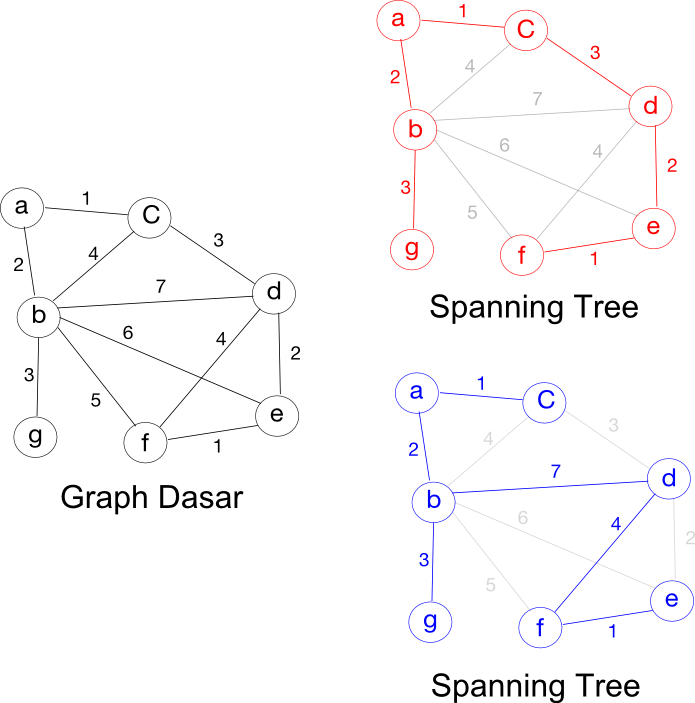
\includegraphics[width=\textwidth,keepaspectratio]{fig/SpanningTreeIntro.png}%
	\caption{Spanning Tree dalam sebuah Graph}%
	\label{fig:spanning-tree-intro}%
\end{figure}

Ketika menggambarkan sebuah Spanning Tree, kita dapat mengalokasikan nilai untuk setiap edge di dalamnya. Total bobot dari keseluruhan edge yang ada di dalam sebuah Spanning Tree kita kenal dengan istilah \textit{weight}. Sebuah Spanning Tree yang memiliki total nilai \textit{weight} terendah kita kenal dengan nama \textbf{Minimum Spanning Tree (MST)}.

MST memiliki banyak aplikasi pada perancangan sistem, terutama untuk sistem-sistem yang berhubungan dengan jaringan. Salah satu contoh pemanfaatan MST yaitu ketika sebuah perusahaan listrik ingin menambahkan jangkauan listrik ke suatu daerah, dengan memasang tiang listrik. Pemasangan tiang listrik pada suatu daerah akan dibatasi oleh berbagai batasan fisik, misalnya perusahaan listrik tidak mungkin memasang tiang listrik di dalam rumah penduduk. Jika kita mengasumsikan pemasangan hanya dilakukan pada sepanjang jalan, kita dapat membangun graph untuk merepresentasikan titik-titik yang dapat menjadi tempat pemasangan tiang listrik. Gambar~\ref{fig:electricity-installation} menggambarkan graph yang mungkin kita bangun untuk pemasangan listrik dalam sebuah kota.

\begin{figure}
    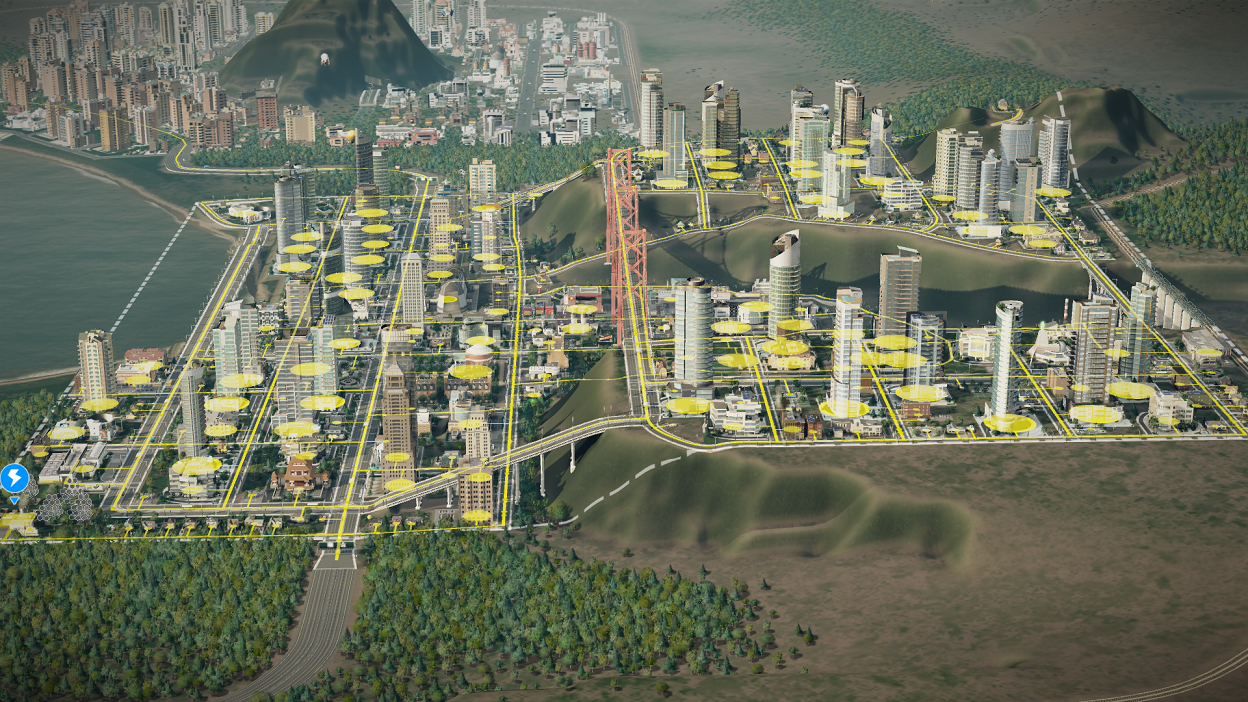
\includegraphics[width=\textwidth,keepaspectratio]{fig/ElectricityInstallation.png}%
	\caption{Jalur Pemasangan Tiang Listrik dalam Graph (Lingkaran Kuning adalah Vertex)}%
	\label{fig:electricity-installation}%
\end{figure}

Ketika sudah memiliki graph untuk jalur pemasangan tiang listrik seperti pada gambar~\ref{fig:electricity-installation}, kita kemudian dapat memberikan bobot kepada masing-masing edge yang ada. Acuan untuk nilai bobot yang digunakan dapat berbeda-beda, tergantung dari tujuan yang ingin dicapai. Contoh dari acuan yang dapat digunakan adalah jarak antar titik. Selain itu, kita juga dapat menggunakan biaya pemasangan sebagai tolak ukur bobot. Pemasangan tiang listrik pada sebuah bukit tentunya akan lebih mahal dan sulit, meskipun mungkin jarak yang ditempuh akan menjadi lebih sedikit.

Setelah memiliki graph pemasangan dan memilih acuan bobot dari edge, kita kemudian dapat mengguankan MST untuk menentukan jalur pemasangan listrik yang paling optimal. Metode pemanfaatan MST yang seperti ini dapat kita terapkan pada berbagai proses lain, seperti pemasangan kabel telepon, segmentasi gambar, dan lain-lain.

\section{Syarat dan Sifat MST}

Berdasarkan kajian singkat yang telah kita bahas pada bagian sebelumnya, terdapat beberapa kesimpulan yang dapat kita tarik. Pertama, sebelum membangun sebuah MST, kita terlebih dahulu harus memiliki dua hal berikut:

\begin{enumerate}
    \item Sebuah Graph satu arah
    \item Bobot dari masing-masing edge di dalam graph
\end{enumerate}

Kedua, sifat-sifat umum yang dimiliki oleh sebuah MST yaitu:

\begin{enumerate}
    \item Sebuah graph dapat memiliki banyak MST
    \item Jika setiap edge yang ada dalam graph memiliki nilai unik, maka hanya akan terdapat satu MST di dalam graph tersebut
    \item Jika bobot dari semua edge selalu bernilai positif, MST yang didapatkan akan selalu merupakan subgraph dengan bobot terkecil yang menghubungkan seluruh vertex
    \item Tidak boleh terdapat siklus (\textit(cycle)) di dalam MST, karena sebuah siklus karena total bobot graph dengan siklus akan selalu lebih besar dari graph tanpa siklus
\end{enumerate}

Pembentukan MST dari sebuah graph sendiri merupakan permasalahan optimasi yang dapat kita selesaikan dengan algoritma greedy. Pada bagian berikutnya kita akan membahas dua buah algoritma umum yang digunakan untuk membangun MST, yaitu algoritma Kruskall dan Prim.

\section{Algoritma Kruskall}

\section{Algoritma Prim}

Algoritma Prim membangun sebuah MST dengan membuat tree dari sebuah graph terlebih dahulu. Tree yang akan dibangun oleh algoritma Prim dimulai dari sebuah vertex acak, yang nantinya akan dibangun satu demi satu vertex untuk menjadi MST. Gambar~\ref{fig:prims-proc} menunjukkan hubungan graph dengan pohon MST yang dibangun dengan algoritma Prim.

\begin{figure}
    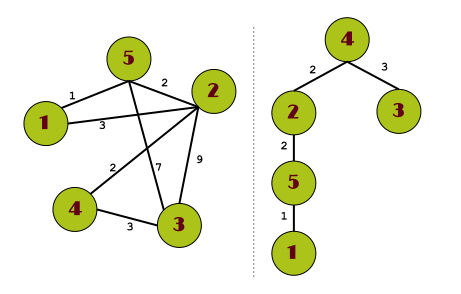
\includegraphics[width=\textwidth,keepaspectratio]{fig/PrimsProc.png}%
	\caption{Kiri: Graph Asal, Kanan: Tree MST dengan Prim}%
	\label{fig:prims-proc}%
\end{figure}

Algoritma Prim membuat tree (selanjutnya disebut sebagai Spanning Tree) karena sebuah Tree tidak mungkin menghasilkan siklus dalam graph. Jika terdapat siklus di dalam graph yang dihasilkan, maka graph tersebut tidak dapat dikatakan sebagai sebuah MST.

Pembangunan Spanning Tree pada algoritma Prim sendiri dilakukan dalam beberapa tahap. Pada tahap pertama, kita menambahkan satu vertex sebagai akar dari Spanning Tree. Vertex manapun dapat dipilih sebagai akar dari Spanning Tree. Untuk iterasi-iterasi berikutnya, kita akan menambahkan vertex baru ke dalam Spanning Tree, sesuai dengan kriteria yang diwajibkan MST, yaitu vertex dengan bobot edge paling kecil dari vertex asal (sebelumnya).

Urutan pengambilan vertex untuk dimasukkan ke dalam Spanning Tree sendiri dapat dilakukan dengan beberapa cara. Misalnya, kita dapat mengambil vertex dengan edge terendah terhadap vertex terakhir di Spanning Tree dengan menandai tiap vertex dengan ukuran jarak. Pendekatan yang lebih pintar dapat memanfaatkan Priority Queue untuk menandai urutan prioritas vertex yang akan dikunjungi.

Agar tidak terlalu bingung, mari kita langsung lihat contoh implementasi algoritma Prim dengan Priority Queue. Fungsi Prim yang akan kita bangun menerima dua parameter, yaitu graph yang akan dicari MST-nya dan vertex awal untuk memulai algoritma Prim:

\lstinputlisting[language=Python, 
                 label={algo:prim-declaration},
                 firstline=3,
                 lastline=3,
                 caption=Deklarasi Fungsi Prim
                ]
                {code/15-prims.py}

Selanjutnya, kita dapat menginisalisasi variabel-variabel awal yang akan kita butuhkan. Variabel pertama yang diinisialisasi adalah $vtx$, yang menyimpan semua vertex asal. $q$ merupakan Priority Queue yang akan menyimpan seluruh vertex beserta tingkat prioritasnya. Untuk menyederhanakan implementasi, Priority Queue akan kita simpan dalam sebuah Dictionary, dengan key berupa vertex dan value berupa nilai prioritas.

Sebagai nilai awal untuk $q$, kita akan mengisikan semua vertex yang ada, dengan prioritas maksimal (sebesar-besarnya). Hal ini dilakukan karena pada awal algoritma, kita belum mengetahui vertex mana yang akan dijalankan terlebih dahulu. Algoritma~\ref{algo:prim-init} menunjukkan langkah yang kita jalankan sejauh ini.

\lstinputlisting[language=Python, 
                 label={algo:prim-init},
                 firstline=4,
                 lastline=8,
                 caption=Deklarasi Variabel Awal Prim
                ]
                {code/15-prims.py}

Selanjutnya, kita dapat membuat Spanning Tree yang akan dibangun, dalam variabel $t$. Sama seperti Priority Queue, kita akan menyimpan pohon di dalam Dictionary, dengan key sebagai nod yang aktif dan vertex sebagai orang tua (\textit{parent}) dari node tersebut. Pada node akar, kita akan mengisikan orang tua dengan nilai None.

Kita juga dapat sekaligus mengisikan nilai awal dari $t$ dan $q$, yaitu vertex awal yang dikirimkan oleh fungsi. Untuk $q$, prioritas vertex awal akan diisikan dengan $0$ agar pada iterasi selanjutnya kita dapat mulai dari vertex ini. Algoritma~\ref{algo:prim-init2} menunjukkan langkah kita sampai titik ini.

\lstinputlisting[language=Python, 
                 label={algo:prim-init2},
                 firstline=10,
                 lastline=13,
                 caption=Inisialisasi Nilai Awal Prim
                ]
                {code/15-prims.py}

Iterasi pembangunan Spanning Tree dapat dilakukan dengan mengambil seluruh tetangga vertex dengan Prioritas Utama (nilai minimum), dan membandingkan bobot edge antara vertex asal dengan seluruh tetangganya. Kita mencari nilai bobot edge yang lebih kecil dari nilai prioritas di sini. Nilai edge terkecil ini diambil karena kita ingin mengambil nilai minimum. Jika edge lebih kecil dari prioritas, kita akan menjadikan nilai edge tersebut nilai prioritas vertex. Nilai prioritas vertex ini akan terus diperbaharui sampai vertex menjadi prioritas terkecil. Hal ini akan otomatis mengeliminasi siklus, karena edge siklus tidak akan dapat menjadi prioritas terkecil; ingat: edge siklus akan selalu lebih besar dari edge non-siklus.

Begitu kita mendapatkan edge dengan prioritas terkecil, kita dapat langsung memasukkannya ke dalam Spanning Tree. Algoritma~\ref{algo:prim-spanning-tree} menunjukkan langkah-langkah yang diambil untuk membangun Spanning Tree.

\lstinputlisting[language=Python, 
                 label={algo:prim-spanning-tree},
                 firstline=15,
                 lastline=25,
                 caption=Pembangunan Spanning Tree
                ]
                {code/15-prims.py}

Setelah mendapatkan Spanning Tree dari algoritma Prim, kita dapat membangun Graph MST-nya dengan cukup mudah: telusuri tree dan bangun node serta edge-nya, seperti yang dilakukan pada Algoritma~\ref{algo:prim-mst}.

\lstinputlisting[language=Python, 
                 label={algo:prim-mst},
                 firstline=27,
                 lastline=33,
                 caption=Pembangunan MST dari Spanning Tree
                ]
                {code/15-prims.py}

Keseluruhan algoritma Prim yang kita bangun dapat dilihat pada Algoritma~\ref{algo:prim-complete}.

\lstinputlisting[language=Python, 
                 label={algo:prim-complete},
                 caption=Algoritma Prim
                ]
                {code/15-prims.py}

%\chapter{Graph}

Graph merupakan sebuah \textit{Abstract Data Type} (ADT) yang digunakan untuk mengimplementasikan konsep \textit{graph} dan \textit{directed graph} dalam matematika. Dalam matematika sendiri, graph merupakan sebuah representasi dari sekumpulan objek yang saling terhubung. Objek-objek yang ada di dalam graph dikenal dengan nama \textit{vertex}, sedangkan hubungan (penghubung) antar objek tersebut dikenal dengan nama \textit{edge}.

Sebuah graph dapat digunakan untuk merepresentasikan banyak hal dalam dunia nyata. Misalnya, kita dapat merepresentasikan pohon pengetahuan dalam sebuah graph seperti yang nampak pada gambar~\ref{fig:knowledge-tree}. Peta juga kerap kali direpresentasikan sebagai graph, dengan titik-titik pergerakan sebagai vertex-nya, dan jalur antar titik sebagai edge-nya (lihat gambar~\ref{fig:map-graph}).

\begin{figure}
    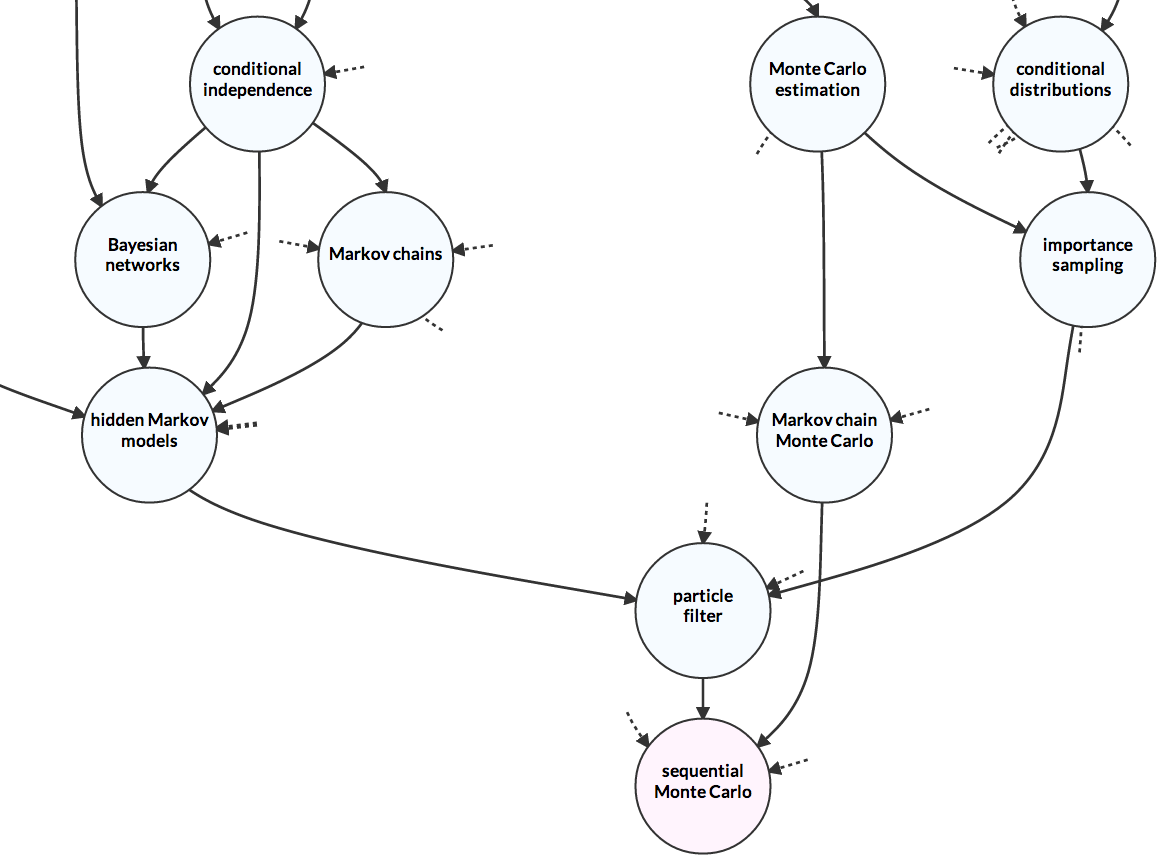
\includegraphics[width=\textwidth,keepaspectratio]{fig/KnowledgeTree.png}%
	\caption{Pohon Pengetahuan}%
	\label{fig:knowledge-tree}%
\end{figure}

\begin{figure}
    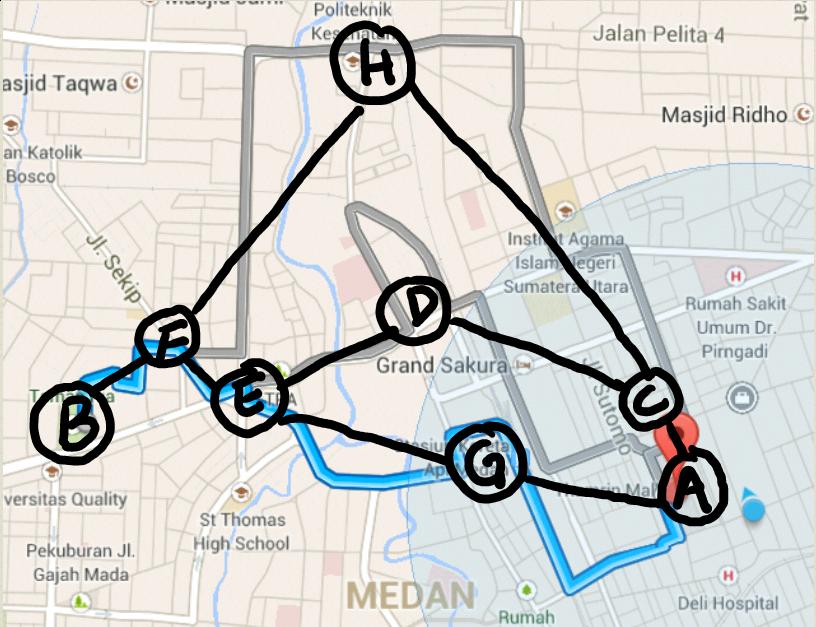
\includegraphics[width=\textwidth,keepaspectratio]{fig/DirectedGraphMap.png}%
	\caption{Peta dengan Graph}%
	\label{fig:map-graph}%
\end{figure}

Terdapat sangat banyak jenis dan definisi dari graph, yang masing-masing memiliki kegunaan spesifik dan kelebihan serta kekurangan tersendiri. Pada bagian ini kita hanya akan membahas satu jenis graph, yaitu graph tidak berarah yang berlabel. Untuk mengetahui lebih lanjut mengenai detil dari berbagai jenis graph serta kelebihan dan kekurangannya, silahkan baca buku atau modul tentang struktur data terkait.

Graph tidak berarah berlabel yang kita gunakan didefinisikan sebagai berikut:

\begin{itemize}
    \item Sebuah graph didefinisikan sebagai $G = (V, E)$.
    \item $V$ merupakan sekumpulan vertex.
    \item $E$ merupakan sekumpulan edge.
    \item $E = (V1, V2, v)$ di mana $V1$ dan $V2$ adalah dua buah vertex yang terhubung dan $v$ adalah label (bobot; jarak) dari kedua vertex tersebut.
    \item Dua buah vertex yang saling berdampingan membentuk sebuah edge dapat dihubungkand engan simbol $~$, sehingga $u ~ v$ dapat dibaca sebagai vertex $u$ dan $v$ yang berdampingan (memiliki edge).
\end{itemize}

Definisi graph yang kita gunakan tidak terlalu jauh berbeda dengan yang digunakan pada teori graph dalam matematika pada umumnya. Tetapi ingat bahwa definisi ini seringkali dimodifikasi sesuai dengan kebutuhan dan tujuan dari algoritma yang menggunakan graph tersebut. Misalnya, representasi dan definisi dari sebuah graph yang digunakan untuk menyelesaikan permasalahan pemetaan seperti mencari jalur terpendek akan berbeda dengan representasi untuk menyelesaikan masalah deteksi bahasa. Begitupun, algoritma-algoritma dasar yang sama dapat kita immplementasikan pada representasi graph yang berbeda ini (misalnya: algoritma untuk pencarian jalur terpendek). Perbedaan hanya akan ditemukan pada detil implementasi nantinya.

Untuk memperjelas pengertian tentang representasi graph yang berbeda, kita akan melihat beberapa jenis cara merepresentasikan graph yang umum digunakan.

\section{Representasi Graph}

Sebagai sebuah struktur data tingkat tinggi, kita umumnya akan membangun graph dengan menggabungkan beberapa struktur data sederhana seperti array, struktur, atau objek. Beberapa struktur data sederhana ini kemudian diintegrasikan dengan aturan tertentu agar dapat direpresentasikan sebagai graph. Secara umum terdapat tiga metode untuk merepresentasikan graph dari struktur-struktur sederhana seperti ini, yaitu:

\begin{description}
    \item[Adjacency List] \hfill \\
        Pada adjacency list, vertex direpresentasikan sebagai sebuah objek khusus (mulai dari yang sederhana seperti string sampai objek buatan sendiri). Vertex kemudian disimpan di dalam sebuah list atau array, dan setiap vertex menyimpan list atau array dari vertex yang berdampingan.
    \item[Adjacency Matrix] \hfill \\
        Pada adjacency matrix, kita menyimpan data graph di dalam sebuah matriks, dengan bagian baris sebagai vertex asal dan bagian kolom sebagai vertex tujuan. Isi dari matriks sendiri adalah jumlah edge yang menghubungkan kedua vertex (baris dan kolom). Data dari semua vertex dan edge sendiri harus di luar matriks.
    \item[Incidence Matrix] \hfill \\
        Pada incidence matrix, graph direpresentasikan dalam matriks dua dimensi, dengan baris matriks sebagai vertex dan kolom matriks sebagai edge. Nilai dari matriks mengindikasikan keterhubungan (\textit{incidence}) antara vertex dengan edge.
\end{description}

Untuk melihat detil yang dijabarkan, mari kita lihat masing-masing representasi ini dengan lebih mendalam.

\subsection{Graph dengan Adjacency List}

Seperti yang telah dijelaskan sebelumnya, pada representasi graph dengan adjacency list, kita terlebih dahulu menyimpan seluruh vertex ke dalam sebuah list. Semua vertex ini kemudian menyimpan sebuah list lagi, yang berisi vertex lain yang berdekatan dengannya. Gambar~\ref{fig:graph-adj-list} mengilustrasikan graph yang direpresentasikan dengan adjacent list.

\begin{figure}[h!]
    \centering
    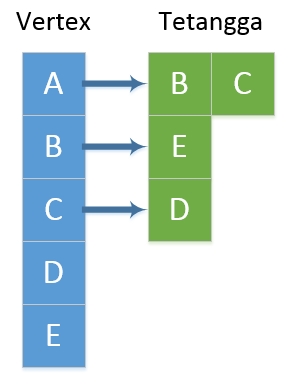
\includegraphics[width=.3\textwidth,keepaspectratio]{fig/Graph-AdjacencyList.png}%
	\caption{Graph dengan Adjacency List}%
	\label{fig:graph-adj-list}%
\end{figure}

\FloatBarrier

Untuk membuat graph dengan adjacency list, kita dapat mulai dengan mentukan objek vertex terlebih dahulu. Dengan asumsi kita merepresentasikan objek vertex sebagai sebuah string sederhana (yang tidak mengandung nilai), kita dapat menyimpan sebuah graph seperti gambar~\ref{fig:graph-adj-list} dengan menggunakan struktur data dictionary sederhana seperti pada algoritma~\ref{algo:graph-dict}.

\lstinputlisting[language=Python, 
                 label={algo:graph-dict},
                 caption=Sebuah Graph dengan Dictionary
                ]
                {code/14-graph-dict.py}

Algoritma~\ref{algo:graph-dict} memperlihatkan bagaimana kita dapat memanfaatkan dictionary dengan aturan tertentu untuk merepresentasikan graph. Adapun aturan yang kita gunakan yaitu:

\begin{itemize}
    \item Kunci dictionary merepresentasikan vertex dari graph.
    \item Setiap kunci (vertex) berisi list.
    \item List yang dimiliki oleh setiap vertex berisi daftar vertex lain yang berdekatan dengannya.
\end{itemize}

Pembentukan graph seperti ini merupakan salah satu implementasi yang paling sederhana, dan sangat mudah diimplementasikan. Jika ingin menghubungkan $v1$ ke $v2$ dan membuat edge $v1 ~ v2$, kita cukup menambahkan $v2$ ke dalam list yang ada pada $v1$. Penyimpanan nilai vertex juga dapat dilakukan dengan menggunakan dictionary jika kita ingin menambahkan nilai di dalam edge. Algoritma~\ref{algo:graph-dict-dict} menunjukkan contoh implementasi jika ingin menyimpan graph berlabel.

\lstinputlisting[language=Python, 
                 label={algo:graph-dict-dict},
                 caption=Graph dengan Adjacency List yang Berlabel
                ]
                {code/15-graph-dict-dict.py}

Pada represenatsi graph dengan adjacency list, kita hanya menyimpan vertex yang berdekatan secara langsung dengan vertex utama saja. Perhatikan bagaimana pada algoritma~\ref{algo:graph-dict-dict} vertex $D$ dan $E$ hanya mengandung list kosong, karena kedua vertex ini tidak memiliki vertex lain didekatnya. Dengan tidak menyimpan data yang tidak diperlukan seperti ini tentunya adjacency list menggunakan memori secara optimal (tidak menyimpan data yang tidakdiperlukan).

Kekurangan utama dari representasi graph dengan adjacency list seperti ini sendiri yaitu untuk pengecekan apakah dua buah vertex saling berdekatan. Karena kita tidak dapat langsung melakukan pengecekan baris-kolom seperti pada adjacency matrix, operasi ini otomatis akan harus dilakukan dengan megecek satu per satu kunci di dalam vertex, yang akhirnya akan memberikan operasi $O(n)$, yang dapat dikatakan lambat dibandingkan dengan operasi $O(1)$ pada adjacency matrix.

\subsection{Graph dengan Adjacency Matrix}

\subsection{Graph dengan Incidence Matrix}

\section{Operasi Umum Graph}

Terdapat beberapa operasi umum yang dapat dilakukan terhadap graph, yaitu:

\begin{enumerate}
    \item Penambahan Vertex baru
    \item Penambahan Edge baru
    \item Penghapusan Vertex
    \item Penghapusan Edge
    \item Pengecekan apakah dua buah vertex terhubung
\end{enumerate}

Kompleksitas dari masing-masing operasi sendiri berbeda-beda, tergantung dari cara representasi graph yang kita gunakan

\section{Contoh Implementasi Graph}

Implementasi graph dapat dimulai dari pembuatan sebuah kelas untuk graph seperti yang dapat dilihat pada algoritma~\ref{algo:migraph-class}.

\lstinputlisting[language=Python, 
                 firstline=1,
                 lastline=1,
                 label={algo:migraph-class},
                 caption=Definisi Kelas MiGraph
                ]
                {code/migraph.py}

Struktur graph sendiri disimpan ke dalam sebuah variabel privat, yang adalah sebuah \textit{dictionary}. Pembuatan struktur internal graph ini dibuat pada saat objek dibuat. Pengguna juga dapat memberikan graph sesuai dengan struktur internal, seperti yang tampak pada algoritma~\ref{algo:migraph-constructor}.

\lstinputlisting[language=Python, 
                 firstline=16,
                 lastline=17,
                 label={algo:migraph-constructor},
                 caption=Definisi Constructor MiGraph
                ]
                {code/migraph.py}

Pengambilan seluruh vertex dan edge yang ada dapat dilakukan dengan cukup gamblang: hanya mengubah kunci dictionary menjadi list untuk vertex, dan menelusuri isi value dari dictionary untuk edges. Algoritma~\ref{algo:migraph-vertices-edges} menunjukkan cara kerja dari bagian pengambilan seluruh vertex dan edge.

\lstinputlisting[language=Python, 
                 firstline=19,
                 lastline=30,
                 label={algo:migraph-vertices-edges},
                 caption=Pengambilan Seluruh Vertex dan Edge
                ]
                {code/migraph.py}

Karena cara penyimpanan adjacent list yang menyimpan semua vertex tetangga di dalam key dictionary, kita dapat mengecek apakah sebuah vertex bertetangga dengan vertex lain dengan sangat mudah. Algoritma~\ref{algo:migraph-is-adjacent} memperlihatkan implementasi fungsi untuk pengecekan apakah vertex bertetangga dengan vertex lainnya.

\lstinputlisting[language=Python, 
                 firstline=32,
                 lastline=33,
                 label={algo:migraph-is-adjacent},
                 caption=Cek Apakah $v1$ dan $v2$ Bertetangga
                ]
                {code/migraph.py}

Penambahan vertex dan edge juga dapat dilakukan dengan sangat sederhana: tambahkan nilai baru di dalam dictionary atau list sesuai dengan kebutuhan. Algoritma~\ref{algo:migraph-add-vertex-edge} memperlihatkan cara implementasi fungsi penambahan vertex dan edge.

\lstinputlisting[language=Python, 
                 firstline=35,
                 lastline=56,
                 label={algo:migraph-add-vertex-edge},
                 caption=Penambahan Vertex dan Edge
                ]
                {code/migraph.py}

Pengambilan vertex yang ada di sekitar vertex sendiri dilakukan dengan cara yang sama dengan pengambilan vertex: hanya mengubah key menjadi list. Algoritma~\ref{algo:migraph-get-neighbour} menunjukkan langkah yang digunakan.

\lstinputlisting[language=Python, 
                 firstline=58,
                 lastline=68,
                 label={algo:migraph-get-neighbour},
                 caption=Pengambilan Vertex Sekitar
                ]
                {code/migraph.py}

Penghapusan vertex maupun edge dilakukan dengan cara yang sama dengan penambahan dan pengambilan nilai vertex, yaitu sesuai dengan semantik python. Algoritma~\ref{algo:migraph-remove-vertex-edge} menunjukkan langkah yang digunakan.

\lstinputlisting[language=Python, 
                 firstline=70,
                 lastline=78,
                 label={algo:migraph-remove-vertex-edge},
                 caption=Penghapusan Vertex dan Edge
                ]
                {code/migraph.py}


%\chapter{Graph Traversal}

Permasalahan paling mendasar dari sebuah graph adalah mengunjungi setiap edge dan vertex dari sebuah graph dalam cara yang sistematik. Untuk menyelesaikan permasalahan tersebut maka kita memerlukan sebuah algoritma graph traversal. Ide dasar dari sebuah graph traversal adalah menandai (marking) setiap vertex yang telah kita kunjungi dan menjelajahi vertex yang belum kita kunjungi.

Pada umumnya, kita beri 3 tanda pada setiap vertex sebagai berikut.
\begin{enumerate}
	\item Belum dikunjungi (\textit{undiscovered}), vertex yang masih dalam kondisi awal. Umumnya ditandai dengan warna putih.
	\item Sudah dikunjungi (\textit{discovered}), vertex yang sudah dikunjungi tetapi masih belum menjelajahi tetangga dari vertex tersebut. Umumnya ditandai dengan warna abu-abu.
	\item Sudah diproses (\textit{processed}), vertex yang sudah dikunjungi dan semua tetangga juga sudah dijelajahi. Umumnya ditandai dengan warna hitam.
\end{enumerate}

Sebuah vertex berubah tanda secara bertahap dari \textit{Undiscovered} menjadi \textit{Discovered} dan terakhir menjadi \textit{Processed}. 

Ada 2 algoritma Graph Traversal yang populer yaitu \textit{Breadth-First Search} dan \textit{Depth-First Search}. Masih ada banyak metode Graph Traversal yang lain tetapi itu tidak dibahas di materi ini. Mahasiswa diharapkan untuk mencari tau jenis-jenis Graph Traversal yang lain.

\section{Breadth-First Search}

\textit{Breadth-First Search} (BFS) merupakan metode Graph Traversal yang paling sederhana dan menjadi dasar dari banyak algoritma graph lainnya seperti algoritma Djikstra untuk mencari jalur terpendek dan algoritma Prim untuk mencari minimum spanning tree.

Diberikan sebuah graph $G = (V,E)$ dan sebuah vertex awal $s$, maka algoritma \textit{Breadth-First Search} akan menjelajahi setiap edge dari G untuk menemukan semua vertex yang bisa dicapai dari $s$. \textit{Breadth-First Search} juga dapat mencari jumlah edge minimal (tanpa menghitung bobot edge) untuk mencapai sebuah vertex tertentu. Algoritma BFS bisa digunakan di graph berarah atau tidak berarah. Kompleksitas waktu dari BFS adalah O(V+E).

Illustrasi BFS bisa dilihat di ~\ref{fig:BFS}.

\begin{figure}
    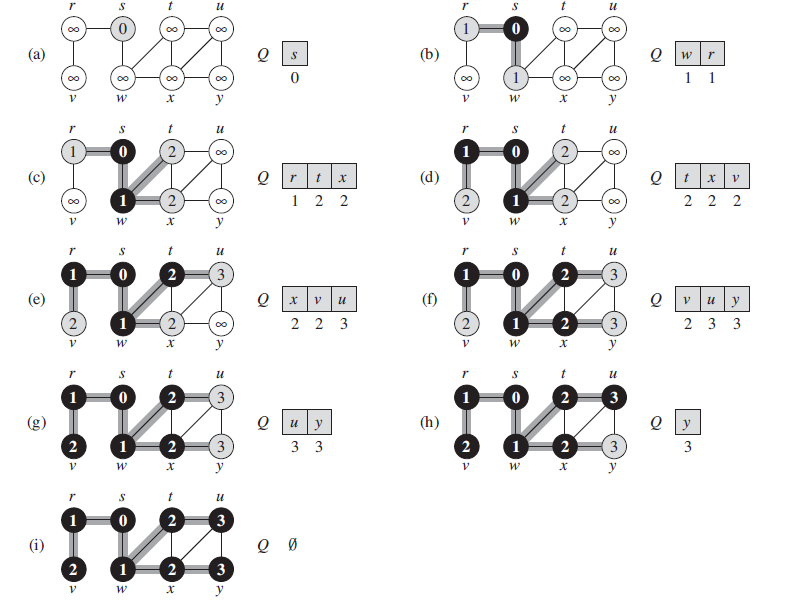
\includegraphics[width=\textwidth,keepaspectratio]{fig/BFS.png}%
	\caption{Illustrasi BFS}%
	\label{fig:BFS}%
\end{figure}

\subsection{Implementasi Breadth-First Search}

Implementasi lengkap dari BFS bisa dilihat dari Algoritma~\ref{algo:migraph-BFS}.

\lstinputlisting[language=Python, 
                 firstline=116,
                 lastline=143,
                 label={algo:migraph-BFS},
                 caption=Implementasi BFS
                ]
                {code/migraph.py}

Fungsi BFS akan menerima satu parameter yaitu vertex sumber $s$ dimana kita akan mulai menjelajahi.

\lstinputlisting[language=Python, 
                 firstline=116,
                 lastline=116,
                 label={algo:migraph-BFS-def},
                 caption=Definisi fungsi BFS
                ]
                {code/migraph.py}

Sebelum memasuki inti dari algoritma BFS, pertama kita deklarasi beberapa variabel untuk BFS yang bisa dilihat di Algo ~\ref{algo:migraph-variabel-BFS}. Variabel $i$, digunakan ketika kita akan mencetak langkah traversal dari BFS. Dengan variabel $i$ kita bisa mengetahui vertex mana yang dikunjungi terlebih dahulu dan selanjutnya. Variabel $traversal$ untuk menyimpan semua urutan kunjungan vertex. Kedua variabel $i$ dan $traversal$ hanya untuk keperluan cetak dan bukan bagian dari BFS. 

Variabel $\_\_color$ digunakan untuk mewarnai setiap vertex yang dikunjungi. Ada tiga warna yaitu $WHITE$, $GRAY$ dan $BLACK$. Variabel $\_\_distance$ untuk mengetahui jarak dari sebuah vertex dari source (vertex awal). Variabel $\_\_predecessor$ untuk mengetahui \textit{predecessor} (parent) dari sebuah vertex. 

\lstinputlisting[language=Python, 
                 firstline=117,
                 lastline=120,
                 label={algo:migraph-variabel-BFS},
                 caption=Variabel BFS
                ]
                {code/migraph.py}

Setelah kita deklarasi, kita definisikan variabel $\_\_color$ dan $\_\_distance$. Semua vertex awalnya berwarna putih dan jaraknya INF. $\_\_predecessor$ tidak usah didefinisikan karena memang nilai awalnya adalah NONE.

\lstinputlisting[language=Python, 
                 firstline=121,
                 lastline=123,
                 label={algo:migraph-define-variabel-BFS},
                 caption=Definisi Variabel BFS
                ]
                {code/migraph.py}

Kita definisikan warna dari vertex $s$ sebagai warna $GRAY$ menandakan vertex sudah dikunjungi tetapi belum semua tetangga dikunjungi dan jarak bernilai 0.

\lstinputlisting[language=Python, 
                 firstline=124,
                 lastline=125,
                 label={algo:migraph-define-s-BFS},
                 caption=Definisi Variabel S BFS
                ]
                {code/migraph.py}

Untuk melacak vertex mana yang sudah dikunjungi kita akan gunakan \textit{Queue} $Q$. Di python, untuk menyederhanakan kita bisa menggunakan \textit{list} yang bisa dilihat di Algo ~\ref{algo:migraph-queue-BFS}. Kita masukkan dulu vertex $s$ ke dalam \textit{Queue} menandakan kita sedang mengunjungi vertex $s$.

\lstinputlisting[language=Python, 
                 firstline=126,
                 lastline=127,
                 label={algo:migraph-queue-BFS},
                 caption=Penggunaan Queue BFS
                ]
                {code/migraph.py}

$Q$ berfungsi sebagai penanda kunjungan kita ke setiap vertex. Semua vertex yang akan kita kunjungi akan kita masukkan dari belakang (\textit{append}) variabel $Q$. Semua tetangga dari vertex $s$ akan kita \textit{append} ke dalam $Q$. Setelah itu kita akan proses dari depan satu persatu. Setiap kita proses satu vertex, kita \textit{append} semua tetangga dari vertex tersebut untuk dikunjungi nanti.

Kita akan looping terus menerus dan lakukan proses di atas sampai semua vertex sudah dikunjungi atau $Q$ tidak berisi lagi (lihat ~\ref{algo:migraph-queue-while-BFS}).

\lstinputlisting[language=Python, 
                 firstline=129,
                 lastline=129,
                 label={algo:migraph-queue-while-BFS},
                 caption=Looping selama masih ada isi di Queue.
                ]
                {code/migraph.py}
								
Di awal dari looping, kita akan mengeluarkan vertex paling depan dari $Q$ untuk diproses. 

\lstinputlisting[language=Python, 
                 firstline=130,
                 lastline=130,
                 label={algo:migraph-queue-pop-BFS},
                 caption=Keluarkan isi vertex yang berada di tempat terdepan Queue.
                ]
                {code/migraph.py}

Kita akan memproses vertex yang dikeluarkan ($u$) jika warna dari vertex $u$ adalah $WHITE$ (artinya belum pernah dikunjungi sebelumnya). Pertama kita akan melihat semua tetangga dari vertex $u$. Setiap tetangga tersebut ($v$) kita akan beri warna $GRAY$ menandakan sudah dikunjungi tetapi belum mengunjungi tetangganya. Kemudian kita tambah jarak vertex tersebut 1 (jarak menandakan jarak dari $s$ ke vertex tersebut). Kemudian kita set \textit{predecessor} dari semua vertex tetangga menjadi $u$. Yang terakhir semua tetangga dimasukkan ke belakang dari $Q$.

\lstinputlisting[language=Python, 
                 firstline=136,
                 lastline=141,
                 label={algo:migraph-queue-process-BFS},
                 caption=Proses vertex yang dikeluarkan dari Queue.
                ]
                {code/migraph.py}

Setelah diproses, vertex $u$ tersebut diberi warna $BLACK$ yang artinya sudah dikunjungi dan semua tetangga juga sudah dikunjungi.

\lstinputlisting[language=Python, 
                 firstline=142,
                 lastline=142,
                 label={algo:migraph-vertex-Black-BFS},
                 caption=Vertex diberi warna hitam.
                ]
                {code/migraph.py}
								
Setiap kali kita memproses sebuah vertex, kita akan simpan ke dalam variabel $traversal$ untuk mencatat kunjungan kita. Baris ini bukan bagian dari BFS tetapi hanya untuk keperluan mencatat saja.

\lstinputlisting[language=Python, 
                 firstline=131,
                 lastline=134,
                 label={algo:migraph-traversal-BFS},
                 caption=Mencatat kunjungan dalam traversal.
                ]
                {code/migraph.py}
								
\section{Depth-First Search}

Strategi dari \textit{Depth-First Search} (DFS) berbeda dari BFS dimana BFS mengunjungi terlebih dahulu semua tetangga, maka DFS mengunjungi satu vertex secara mendalam sampai tidak bisa dikunjungi lagi baru pindah ke tetangga baru. Kompleksitas waktu dari DFS sama seperti BFS, O(V+E), akan tetapi untuk graph yang sangat besar sekali DFS bisa terlalu dalam menjelajahi satu verteks tanpa menjelajahi verteks lain.

Illustrasi DFS bisa dilihat di ~\ref{fig:Dfs}.

\begin{figure}
    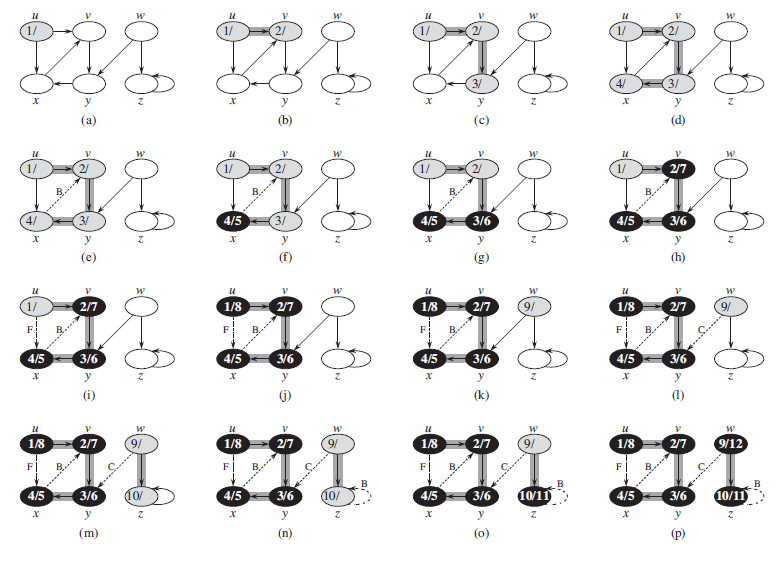
\includegraphics[width=\textwidth,keepaspectratio]{fig/DFS.png}%
	\caption{Illustrasi DFS}%
	\label{fig:Dfs}%
\end{figure}


\subsection{Implementasi Depth-First Search}

Implementasi lengkap dari BFS bisa dilihat dari Algo~\ref{algo:migraph-DFS}. Algoritma dari DFS merupakan algoritma rekursif.

\lstinputlisting[language=Python, 
                 firstline=88,
                 lastline=115,
                 label={algo:migraph-DFS},
                 caption=Implementasi DFS
                ]
                {code/migraph.py}

Pada fungsi $DFS\_traversal(s)$, semua verteks akan diwarnai dengan warna $WHITE$ terlebih dahulu. Setelah itu kita akan mulai mengunjungi dari vertex $s$. Kunjungan akan ditandai dengan memanggil fungsi $DFS\_visit$

\lstinputlisting[language=Python, 
                 firstline=88,
                 lastline=98,
                 label={algo:migraph-DFS-2},
                 caption=Implementasi DFS
                ]
                {code/migraph.py}

Fungsi $DFS\_visit$ akan mengunjungi semua vertex beserta anaknya sampai yang paling dalam. Inti dari DFS adalah pada rekursif, dimana setiap tetangga vertex $v$ yang berwarna $WHITE$ akan dikunjungi dan ketika rekursif selesai, vertex $v$ tersebut akan diwarnai $BLACK$.

\lstinputlisting[language=Python, 
                 firstline=99,
                 lastline=114,
                 label={algo:migraph-DFS-3},
                 caption=Implementasi DFS
                ]
                {code/migraph.py}


\chapter{Pemrosesan String}

\section{Pengenalan}

String merupakan sebuah deretan simbol yang bisa dituliskan dengan menggunakan notasi $a_1 a_2 \ldots a_k$, atau $(a_1, a_2, \ldots , a_k)$. Pemrosesan String sangat berguna dalam berbagai aplikasi seperti pemrosesan genom, sistem komunikasi, pemrosesan informasi, dan sebagainya. Ada beberapa struktur data dan algoritma yang harus dipahami terlebih dahulu sebelum melakukan pemrosesan string.  

\section{Struktur Data yang Berkaitan dengan String}
Struktur data yang akan dibahas adalah \textit{Trie}, \textit{Suffix trie}, \textit{Suffix tree} dan \textit{Suffix array}.

\subsection{\textit{Trie}}
\textit{Trie} merupakan singkatan dari kata \textit{reTRIEval} dan merupakan sebuah varian dari pohon pencarian. \textit{Trie} terdiri dari satu atau lebih \textit{node} (\textit{vertex}). Setiap \textit{node} memiliki hubungan (\textit{link}) ke \textit{node} lain ataupun null. Setiap \textit{node} memiliki satu \textit{parent node} dan setiap \textit{node} memiliki satu atau beberapa \textit{link} (\textit{edge}). Contoh dari Trie bisa dilihat di Gambar ~\ref{fig:trie}.

\begin{figure}
    \includegraphics[width=\textwidth,keepaspectratio]{fig/Trie.png}%
	\caption{Pohon Pengetahuan}%
	\label{fig:trie}%
\end{figure}

Gambar \ref{fig:trie} dibentuk dari 4 buah string yaitu: $makan$ bernilai 10, $masak$ bernilai 14, $minum$ bernilai 20 dan $tidur$ bernilai 11. Untuk mencari string $makan$, maka pencarian dimulai dari huruf awal yaitu $m$, kemudian diikuti oleh $a$, $k$, $a$, dan $n$ sampai menemukan nilai 10. Proses pencarian bisa dilihat di Gambar ~\ref{TrieSearchingMakan}.

\begin{figure}
    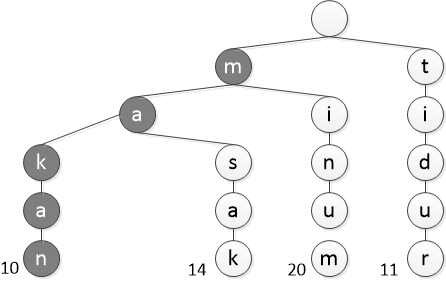
\includegraphics[width=\textwidth,keepaspectratio]{fig/TrieSearchingMakan.png}%
	\caption{Mencari kata $makan$ di Trie}%
	\label{fig:TrieSearchingMakan}%
\end{figure}

Pencarian \textit{node} akan berakhir apabila tidak ada \textit{node} yang cocok dengan kata pencarian kita, atau menemukan kata yang kita cari. Akan tetapi, walaupun kita sudah menemukan kata yang dicari, apabila tidak ada nilai dalam \textit{node} tersebut maka itu akan dianggap tidak ketemu. 

Contohnya jika kita mencari kata $maka$, akan ditemukan di jalur $makan$ tetapi tidak ada ditemukan nilai (null) di akhir pencarian maka kata $maka$ akan dianggap tidak ada di dalam $trie$.

\begin{figure}
    \includegraphics[width=\textwidth,keepaspectratio]{fig/TrieSearchingMaka.png}%
	\caption{Kata $maka$ ditemukan tetapi tidak memiliki nilai (bernilai null).}%
	\label{fig:TrieSearchingMaka}%
\end{figure}

Contoh lain, jika kita mencari kata $makin$, maka kita akan berhenti di huruf $k$ dan tidak bisa meneruskan lagi sehingga dianggap kata $makin$ tidak terdapat di trie.

\begin{figure}
    \includegraphics[width=\textwidth,keepaspectratio]{fig/TrieSearchingMakin.png}%
	\caption{Pencarian berhenti di huruf $k$ dan tidak bisa diteruskan sehingga kata $makin$ tidak ditemukan di trie.}%
	\label{fig:TrieSearchingMakin}%
\end{figure}

Pembentukan \textit{trie} dilakukan dengan menambahkan setiap string ke \textit{trie} dengan langkah berikut.
\begin{enumerate}
	\item Menggunakan karakter pertama dari string sebagai panduan untuk memasukkan ke \textit{trie}. Jika karakter sudah ada di \textit{trie} berupa \textit{node} maka gunakan \textit{node} tersebut untuk merepresentasikan karakter tersebut. Lanjutkan dengan karakter selanjutnya dari string.
	\item Jika tidak ada karakter yang ingin kita masukkan di \textit{trie} maka bentuk node baru.
	\item Apabila semua karakter sudah dimasukkan ke trie, masukkan nilai (\textit{value}) dari string ke karakter terakhir.
\end{enumerate}

Sebagai contoh, kita akan membentuk sebuah \textit{trie} dengan menggunakan string berikut: $she, sells, sea, shells, by, the, sea, shore$.

\begin{enumerate}
	\item Pertama masukkan string $she$. Karena belum ada \textit{node} dengan karakter awal $s$ maka, kita akan bentuk \textit{node} baru untuk semua string $she$. Kemudian berikan nilai 0 di akhir string $she$.
		\begin{figure}
			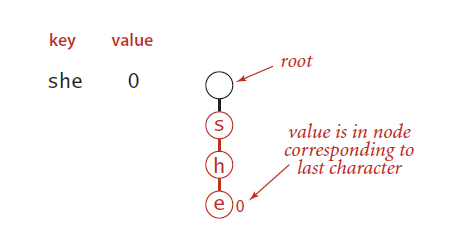
\includegraphics[width=\textwidth,keepaspectratio]{fig/FormTrie1.png}%
			\caption{String $she$ dimasukkan ke dalam Trie.}%
			\label{fig:FormTrie1}%
		\end{figure}
	\item Setelah string $she$, maka selanjutnya adalah string $sells$. Dalam memasukkan string $sells$, karakter pertama yaitu $s$ sudah dimasukkan, untuk itu \textit{node} untuk $s$ yang digunakan oleh $she$ juga digunakan untuk $sells$. Akan tetapi, karakter selanjutnya yaitu $e$ tidak ada setelah $s$ maka itu dibentuk node baru untuk $e$. Kemudian berikan nilai 1 di akhir $sells$.
		\begin{figure}
			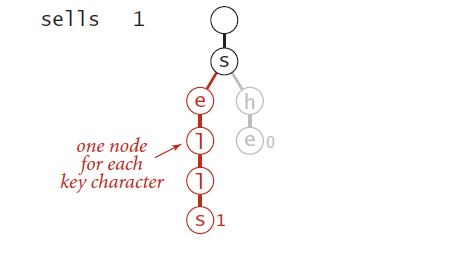
\includegraphics[width=\textwidth,keepaspectratio]{fig/FormTrie2.png}%
			\caption{String $sells$ dimasukkan ke dalam Trie.}%
			\label{fig:FormTrie2}%
		\end{figure}
	\item Lakukan hal yang sama untuk semua string yang tersisa.
		\begin{figure}
			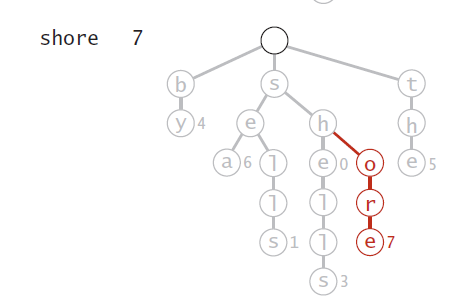
\includegraphics[width=\textwidth,keepaspectratio]{fig/FormTrie3.png}%
			\caption{Semua string dimasukkan ke dalam Trie.}%
			\label{fig:FormTrie3}%
		\end{figure}
\end{enumerate}

\subsection{Implementasi Python}

Untuk implementasi di python, akan menggunakan \textit{dictionary} sebagai dasar dari \textit{Trie}. Kita akan membuat sebuah \textit{class} \textit{Trie} yang terdapat beberapa metode seperti penambahan, penghapusan, dan sebagainya.

Kita akan melihat inisialisasi dari kelas \textit{Trie} yang dapat dilihat di Algoritma ~\ref{algo:trieinit}.
Dalam inisialisasi Trie tersebut variabel $path$ merupakan \textit{dictionary} yang akan menyimpan semua \textit{node} dari Trie. Sedangkan variabel $value$ akan menyimpan nilai dari \textit{node} tersebut. Variabel $value\_valid$ akan menyimpan data boolean yang menandakan apakah \textit{node} tersebut valid atau tidak.

\lstinputlisting[language=Python, 
                 firstline=1,
                 lastline=6,
                 label={algo:trieinit},
                 caption=Inisialisasi Kelas Trie
                ]
                {code/trie.py}
								
Untuk penambahan string baru bisa menggunakan metode di Algoritma ~\ref{algo:trieAdd}. 

\lstinputlisting[language=Python, 
                 firstline=8,
                 lastline=21,
                 label={algo:trieAdd},
                 caption=Penambahan String baru ke Trie
                ]
                {code/trie.py}

Dalam Algoritma ~\ref{algo:trieAdd}, pertama karakter awal dari string akan dimasukkan ke dalam variabel $head$. 

\lstinputlisting[language=Python, 
                 firstline=9,
                 lastline=9,        
                ]
                {code/trie.py}
								
Kemudian, kita akan mengecek apakah sebelumnya sudah ada karakter tersebut di dalam \textit{Trie}. Jika ada maka kita akan mulai dari \textit{node} yang berisikan karakter tersebut. Jika tidak, maka kita akan bentuk \textit{node} baru.

\lstinputlisting[language=Python, 
                 firstline=10,
                 lastline=14,        
                ]
                {code/trie.py}

Setelah itu kita cek apakah karakter yang kita masukkan merupakan yang terakhir dari string. Jika merupakan karakter terakhir maka kita akan akhiri dengan menset \textit{value} dari \textit{node} tersebut. Jika masih tersisa karakter lain, maka kita akan secara rekursif untuk memproses karakter lainnya.

\lstinputlisting[language=Python, 
                 firstline=16,
                 lastline=21,        
                ]
                {code/trie.py}

Untuk penghapusan, kita akan menggunakan metode di ~\ref{algo:trieremove}. 

\lstinputlisting[language=Python, 
                 firstline=23,
                 lastline=34,
                 label={algo:trieremove},
                 caption=Penghapusan node di Trie
                ]
                {code/trie.py}
								
Seperti penambahan, penghapusan string akan dimulai dengan pengecekan karakter pertama apakah ada di dalam \textit{trie} atau tidak.

\lstinputlisting[language=Python, 
                 firstline=24,
                 lastline=25,        
                ]
                {code/trie.py}

Jika ada dalam \textit{trie} maka, kita bisa menghapus string tersebut dengan menggunakan rekursif. 

\lstinputlisting[language=Python, 
                 firstline=26,
                 lastline=34,        
                ]
                {code/trie.py}

Untuk mengambil \textit{value} dari sebuah string, kita bisa menggunakan metode di ~\ref{algo:Trieget} dimana proses pengambilan \textit{value} dilakukan dengan rekursif sampai karakter terakhir untuk mengambil nilainya.

\lstinputlisting[language=Python, 
                 firstline=36,
                 lastline=51,
                 label={algo:Trieget},
                 caption=Mengambil \textit{value} node di Trie
                ]
                {code/trie.py}

Untuk mengecek apakah sebuah string ada atau tidak di dalam Trie bisa menggunakan metode di Algoritma ~\ref{algo:Triecontain}

\lstinputlisting[language=Python, 
                 firstline=36,
                 lastline=51,
                 label={algo:Triecontain},
                 caption=Mengecek apakah sebuah string ada atau tidak di Trie
                ]
                {code/trie.py}
								
Untuk mengambil semua string di Trie dengan prefix tertentu atau semuanya bisa menggunakan metode di Algoritma ~\ref{algo:Triekeys}.

\lstinputlisting[language=Python, 
                 firstline=36,
                 lastline=51,
                 label={algo:Triekeys},
                 caption=Mengambil semua string di Trie
                ]
                {code/trie.py}

\subsection{\textit{Suffix Trie}}

\textit{Suffix Trie} adalah sebuah \textit{Trie} biasa dimana isi dari \textit{Trie} tersebut adalah semua \textit{suffix} dari sebuah string. Sebagai contoh untuk string $abaaba$, maka kita bisa membentuk suffix berupa: $abaaba\$$, $baaba\$$, $aaba\$$, $aba\$$, $ba\$$, $a\$$, dan $\$$. Semua itu akan dibentuk sebuah \textit{trie} yang bisa dilihat di Gambar ~\ref{fig:suffixTrie}

	\begin{figure}
		\includegraphics[width=\textwidth,keepaspectratio]{fig/suffixTrie.png}%
		\caption{Sebuah \textit{suffix trie} dari string $abaaba$.}%
		\label{fig:suffixTrie}%
	\end{figure}

Implementasi dari \textit{Suffix Trie} sama seperti \textit{Trie} biasa hanya saja kita harus mencari dulu semua suffix dari sebuah string baru dimasukkan ke dalam \textit{Trie}. Untuk mencari semua suffix cukup iterasi dari awal string sampai akhir string dan potong satu karakter dari depan setiap kali iterasi.

Dengan menggunakan \textit{suffix trie}, banyak operasi pada string bisa dilakukan dengan cepat. \textit{Suffix trie} lebih efisien dalam penyimpanan dibandingkan dengan menyimpan dalam array biasa. Salah satu contoh pemanfaatan \textit{Suffix Trie} adalah mencari apakah sebuah substring merupakan bagian dari sebuah string misalnya: apakah substring $baa$ merupakan bagian dari $abaaba$? Untuk penyelesaiannya bisa dilihat di Gambar ~\ref{fig:suffixtriefindbaa}. Waktu yang diperlukan untuk mencari adalah sepanjang ukuran query atau O(|query|).

	\begin{figure}
		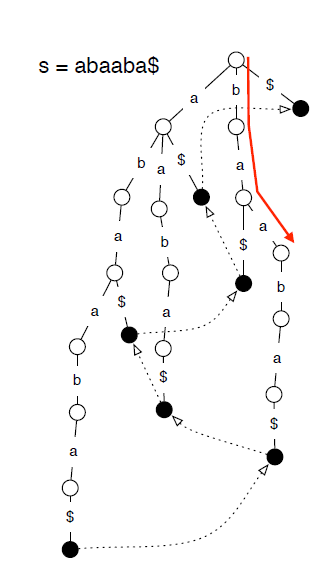
\includegraphics[width=\textwidth,keepaspectratio]{fig/suffixtriefindbaa.png}%
		\caption{Mencari substring $baa$ di string $abaaba$.}%
		\label{fig:suffixtriefindbaa}%
	\end{figure}

Ada banyak apalikasi lain untuk \textit{suffix trie} seperti:
\begin{enumerate}
	\item Mencari apakah sebuah string merupakan suffix dari string lain.
	\item Mencari \# kemunculan dari sebuah string dalam string lain.
	\item Mencari jumlah substring yang paling banyak muncul di sebuah string.
\end{enumerate}

\subsection{\textit{Suffix Tree}}

\textit{Suffix Tree} adalah pengembangan dari \textit{Suffix Trie} dimana semua \textit{node} yang tidak memiliki cabang dikompress menjadi satu \textit{node}. Lihat Gambar ~\ref{fig:suffixtree} untuk melihat \textit{suffix tree} dari string $abaaba$.

	\begin{figure}
		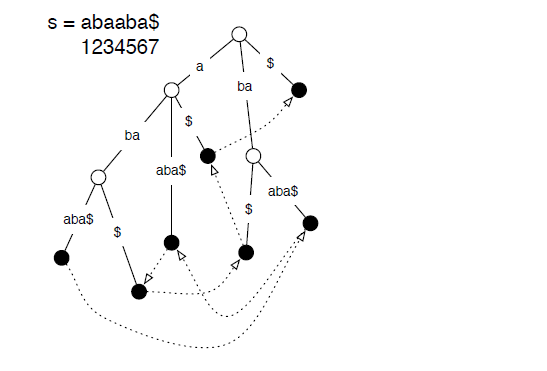
\includegraphics[width=\textwidth,keepaspectratio]{fig/suffixtree.png}%
		\caption{Suffix tree dari string $abaaba$. Perhatikan bahwa pohon menjadi lebih kecil dan lebih ruang efisien}%
		\label{fig:suffixtree}%
	\end{figure}
	
\subsection{\textit{Suffix Array}}

\textit{Suffix Array} merupakan \textit{Suffix Tree} yang disimpan di dalam sebuah array. Semua suffix dari sebuah string disimpan dalam array. Posisi setiap suffix dalam array sesuai dengan urutan \textit{lexicographic} (diurut berdasarkan alphabet setelah diurut berdasarkan panjang suffix). Lihat Gambar ~\ref{fig:suffixarray} untuk melihat \textit{Suffix Array} dari string $abaaba$.

	\begin{figure}
		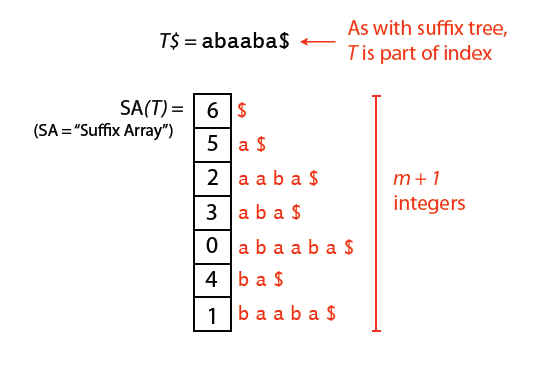
\includegraphics[width=\textwidth,keepaspectratio]{fig/suffixarray.png}%
		\caption{Suffix array dari string $abaaba$.}%
		\label{fig:suffixarray}%
	\end{figure}
	
Implementasi \textit{Suffix Array} adalah yang termudah dari semua. Lihat Algoritma ~\ref{algo:SuffixArray} untuk implementasi \textit{suffix array}.

\lstinputlisting[language=Python, 
                 firstline=4,
                 lastline=9,
                 label={algo:SuffixArray},
                 caption=Membentuk suffix array
                ]
                {code/suffixArray.py}

Untuk \textit{Suffix Array}, kita akan menggunakan \textit{OrderedDict} yang merupakan bagian dari \textit{collections}. Dengan \textit{dictionary} biasa kita tidak bisa mengurut isi dari \textit{dictionary}, akan tetapi dengan \textit{OrderedDict} kita bisa mengurut berdasarkan kunci. 

\section{Algoritma Pemrosesan String}

Untuk pemrosesan String terdapat banyak algoritma, kita akan melihat beberapa contoh algoritma yang bisa memanfaatkan \textit{suffix array}. Kita memilih menggunakan \textit{suffix array} dikarenakan implementasi \textit{suffix array} adalah yang paling mudah dibandingkan dengan \textit{suffix trie} dan \textit{suffix tree}.

\subsection{Pencarian \textit{pattern} Substring dalam String (\textit{String Matching})}

Dengan menggunakan \textit{Suffix Array} dari string $T$, kita bisa mencari \textit{pattern} string $P$ (dengan panjang $m$) dari string $T$ (panjang $n$) tersebut. Pencarian dengan menggunakan \textit{suffix array} lebih mudah dikarenakan 2 hal berikut.

\begin{enumerate}
	\item Jika seandainya $P$ adalah substring dari $T$, maka $P$ harus merupakan \textit{prefix} dari salah satu {suffix} $T$. 
	\item Karena dalam \textit{suffix array}, semua \textit{suffix} sudah diurut berdasarkan \textit{lexicography} maka pencarian \textit{prefix} lebih sederhana. Kita cukup mencocokkan setiap huruf dari urutan pertama dalam \textit{suffix array} sampai urutan terakhir secara berturut. 
\end{enumerate}

Cara naif untuk mencari \textit{pattern} substring dalam sebuah string dalam \textit{suffix array} adalah menggunakan pencarian sekuensial untuk mencocokkan \textit{prefix} dari semua \textit{suffix} yang ada dalam \textit{suffix array}. Untuk illustrasi bisa dilihat di Gambar ~\ref{fig:searchABSuffixArraySequential}.

	\begin{figure}
		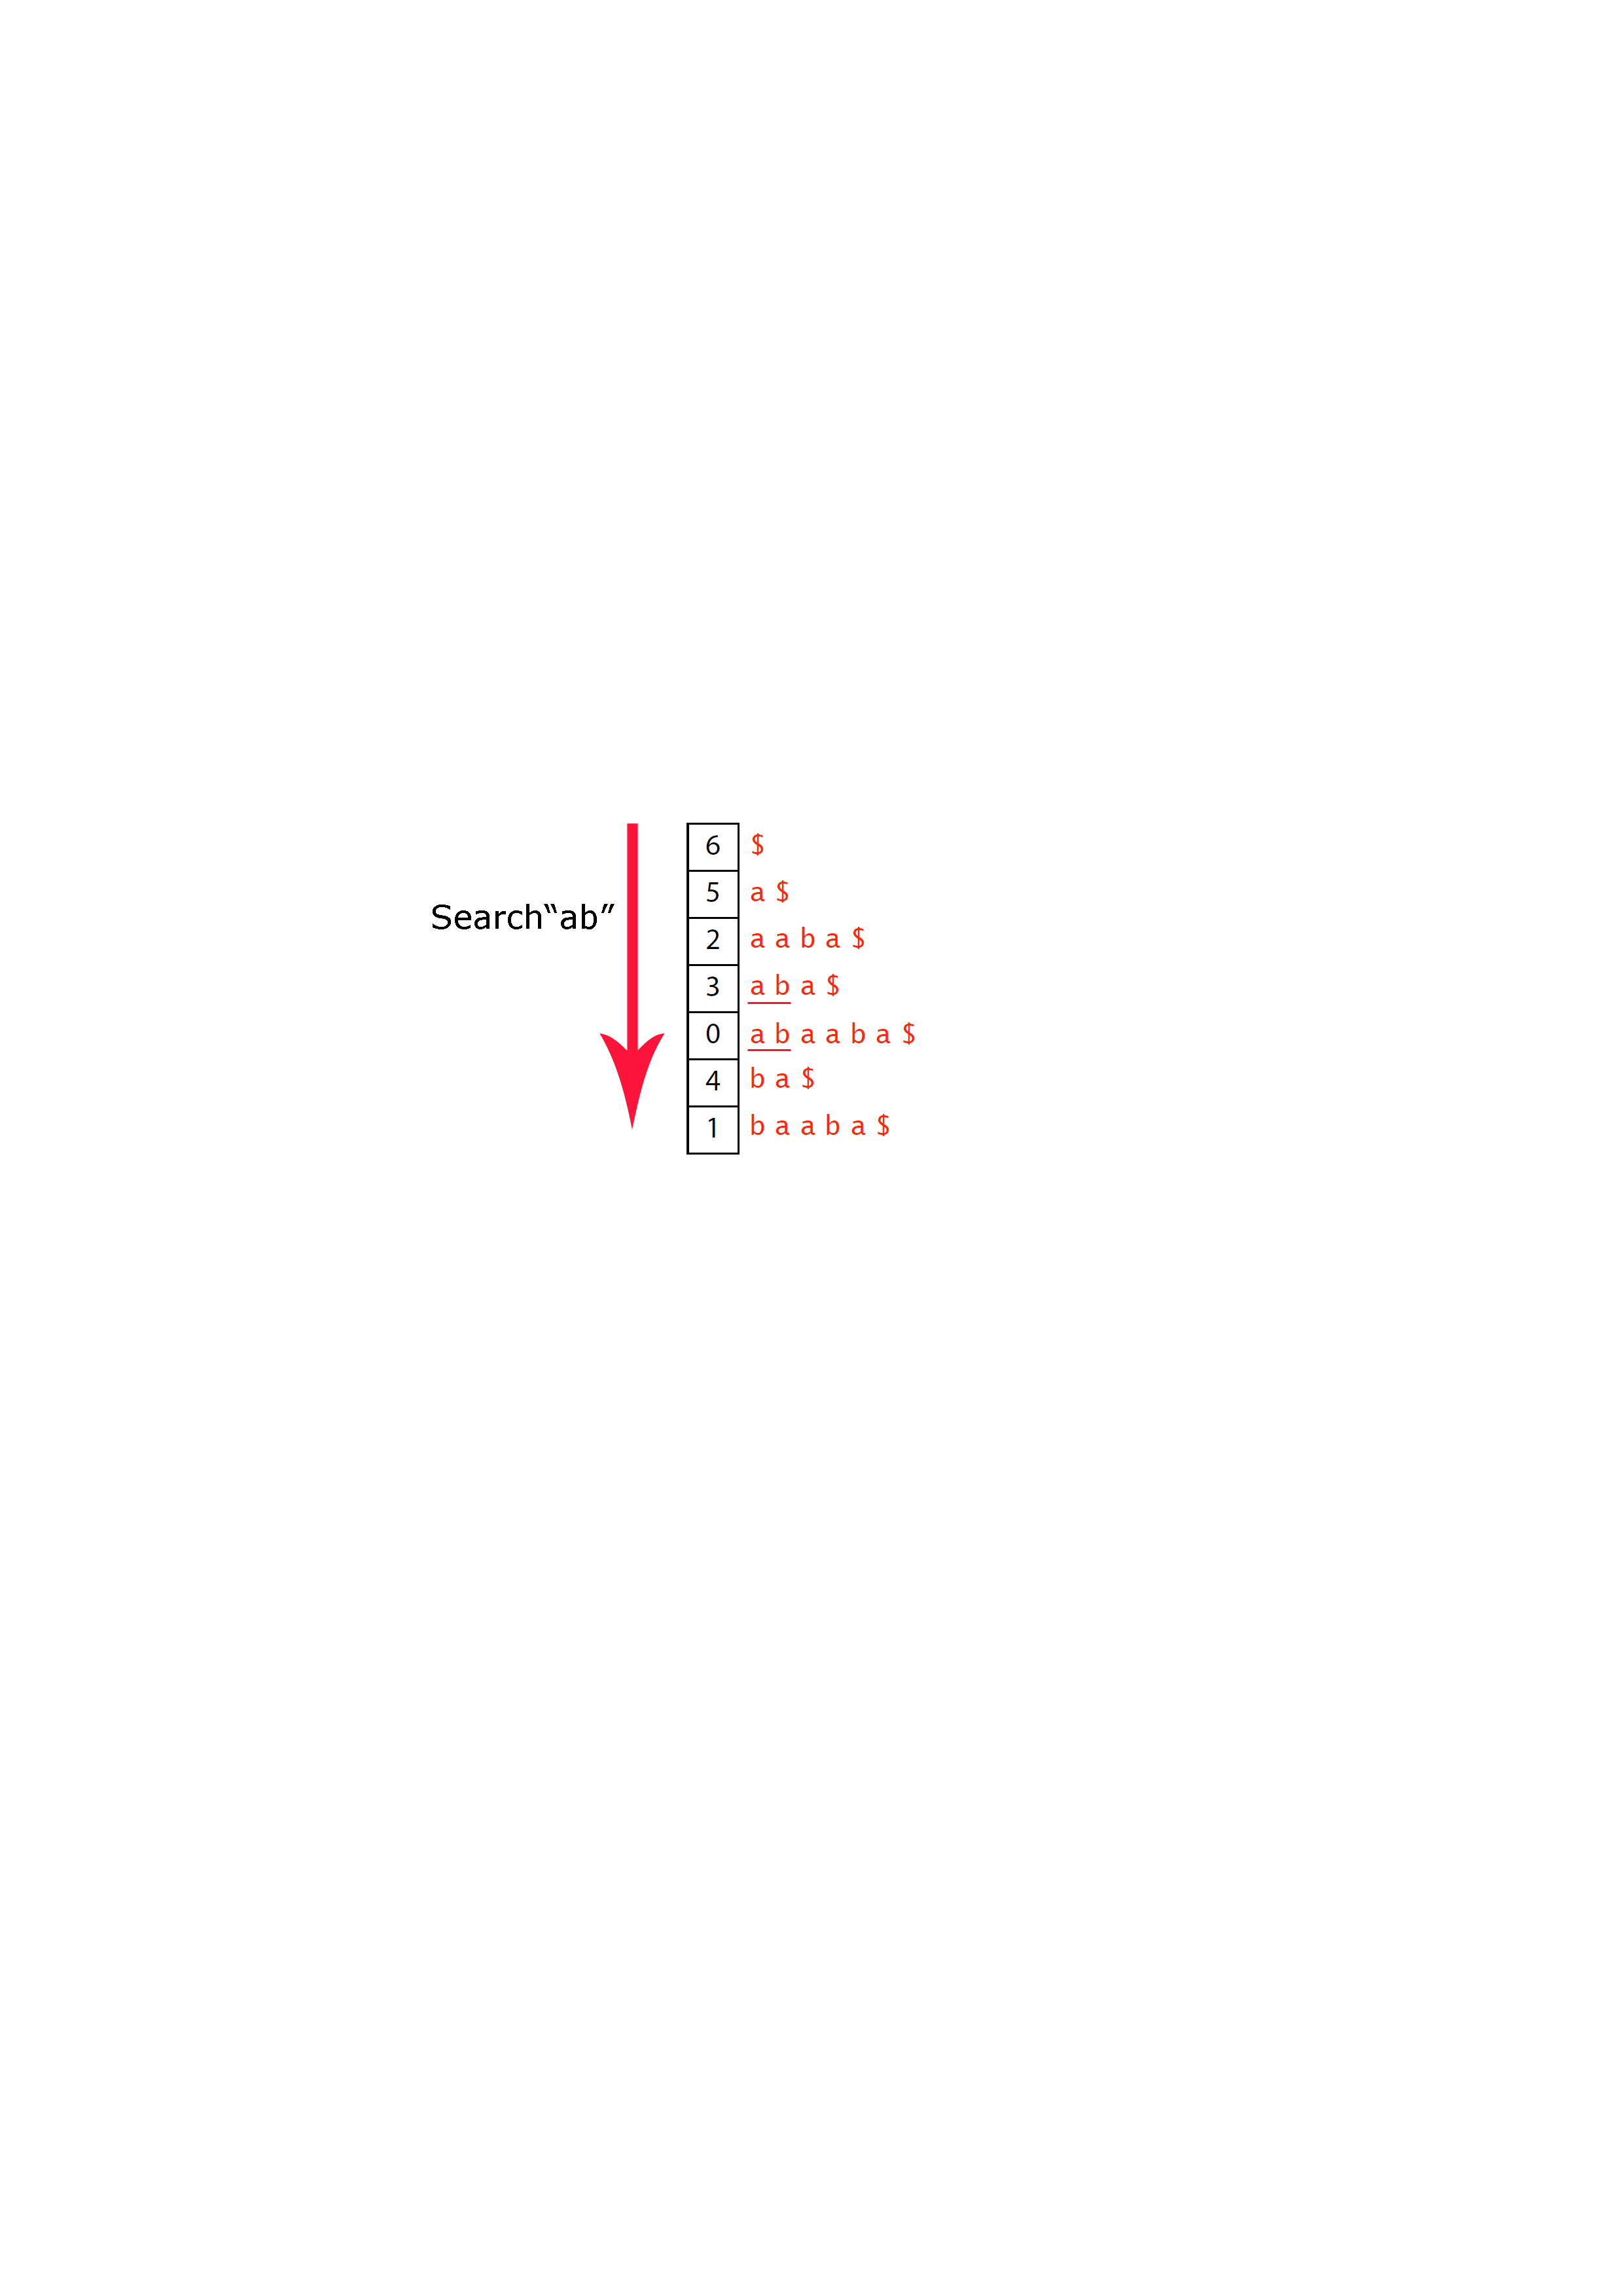
\includegraphics{fig/searchABSuffixArraySequential.png}%
		\caption{Mencari \textit{pattern} $ab$ dari string $abaaba$}%
		\label{fig:searchABSuffixArraySequential}%
	\end{figure}

Untuk implementasi pada Python bisa dilihat di Algoritma ~\ref{algo:StringMatchingNaif}.

\lstinputlisting[language=Python, 
                 firstline=11,
                 lastline=16,
                 label={algo:StringMatchingNaif},
                 caption=\textit{String Matching} naif dengan suffix array
                ]
                {code/suffixArray.py}


Untuk mempercepat pencarian, daripada menggunakan pencarian sekuensial kita akan menggunakan dua kali \textit{Binary Search} untuk mencari di bagian batas bawah dan batas atas. Waktu yang dibutuhkan untuk mencari adalah $O(m log n)$. Implementasi dari penggunaan \textit{Binary Search} bisa dilihat di Algoritma ~\ref{algo:StringMatchingBS}. 

\lstinputlisting[language=Python, 
                 firstline=18,
                 lastline=47,
                 label={algo:StringMatchingBS},
                 caption=\textit{String Matching} suffix array dengan Binary Search
                ]
                {code/suffixArray.py}

Cara kerja dari Algoritma ~\ref{algo:StringMatchingBS} bisa dilihat dari Gambar \ref{fig:StringMatchingBS} dimana kita akan mencari substring $GA$ dalama $GATAGACA$.

	\begin{figure}
		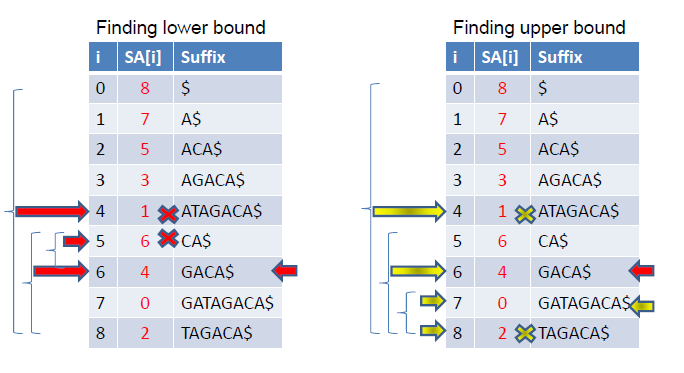
\includegraphics[width=\textwidth,keepaspectratio]{fig/StringMatchingBS.png}%
		\caption{\textit{String matching} dengan \textit{Binary Search}.}%
		\label{fig:StringMatchingBS}%
	\end{figure}
	
Perlu diketahui, bahwa berbeda dengan menggunakan pencarian sekuensial, kita tak perlu mencocokkan satu per satu setiap suffix dalam string $GATAGACA$. Melainkan kita hanya perlu mencari suffix pertama dan suffix terakhir dari string tersebut yang memuat substring $GA$. Sebagai contohnya, dari gambar kita mendapatkan suffix pertama yang memuat $GA$ adalah suffix posisi ke 6 (i=6) yaitu $GATAGACA$, dan suffix terakhir adalah suffix posisi ke 7 (i=7) yaitu $GACA$, maka secara otomatis semua suffix dalam posisi ke 6 dan ke 7 adalah suffix yang memuat $GA$ (karena posisi berdekatan maka hanya ada dua, coba lakukan sekali lagi dengan pencarian substring $A$).

Untuk mencari suffix pertama dan terakhir dibutuhkan dua kali \textit{Binary Search}. Satu untuk mencari yang pertama (\textit{lower bound}) dan satu lagi untuk mencari yang terakhir (\textit{upper bound}).

Untuk mencari suffix pertama kita akan menggunakan \textit{Binary Search} yang bisa dilihat di Algoritma ~\ref{algo:StringMatchingBS1}.

\lstinputlisting[language=Python, 
                 firstline=21,
                 lastline=29,
                 label={algo:StringMatchingBS1},
                 caption=\textit{Binary Search I} untuk mencari suffix pertama yang memuat substring
                ]
                {code/suffixArray.py}

Setelah kita menggunakan \textit{Binary Search} untuk mencari suffix pertama, kita akan mengecek apakah di posisi tersebut ada terdapat substring yang kita inginkan tidak. Jika tidak kita akan mengembalikan -1. Untuk pengecekan lihat di Algoritma ~\ref{algo:StringMatchingNF} 

\lstinputlisting[language=Python, 
                 firstline=30,
                 lastline=31,
                 label={algo:StringMatchingNF},
                 caption=Mengecek apakah di posisi tersebut terdapat substring yang kita inginkan atau tidak.
                ]
                {code/suffixArray.py}

Untuk mencari suffix kedua kita juga akan menggunakan \textit{Binary Search} yang bisa dilihat di Algoritma ~\ref{algo:StringMatchingBS2}.

\lstinputlisting[language=Python, 
                 firstline=21,
                 lastline=29,
                 label={algo:StringMatchingBS2},
                 caption=\textit{Binary Search II} untuk mencari suffix kedua yang memuat substring
                ]
                {code/suffixArray.py}



\subsection{Pencarian pattern terpanjang yang berulang di dalam string}

Diberikan sebuah string $T$, kita ingin mencari pattern $P$ terpanjang yang berulang (minimal >1) dalam string $T$. Misalnya: dalam string $banana$, maka pattern terpanjang yang berulang adalah $ana$.

Untuk menyelesaikan masalah tersebut, kita memerlukan sebuah struktur data yang lebih efisien dan merupakan pengembangan dari \textit{suffix array} yaitu \textit{longest common prefix suffix array} (LCPA. Dalam LCPA, semua panjang LCP akan dihitung dan disimpan dalam \textit{suffix array}. Definisi dari LCP adalah: ``Diberikan dua buah string yaitu $u$ dan $v$, maka prefix terpanjang yang terdapat di kedua buah string tersebut adalah LCP''. Sebagai contohnya:

LCP dari string $\textbf{a}$ dan $\textbf{a}abba$ adalah $a$ dengan panjang 1.

LCP dari string $\textbf{ab}aaabba$ dan $\textbf{ab}ba$ adalah $ab$ dengan panjang 2.

Sebagai contoh dari LCPA, kita bisa melihat contoh berikut dari string $banana$.


\begin{center}
  \begin{tabular}{ | c | c | c |c | c | c | c | c | }
    \hline
    i	& 1	& 2	& 3	& 4	& 5	& 6	& 7 \\ \hline
		A[i]	& 7	& 6	& 4	& 2	& 1	& 5	& 3 \\ \hline
		H[i]	& null	& 0 & 1 &	3 & 0 & 0 & 2 \\ \hline
		1	& \$	& a	& a	& a	& b	& n	& n \\ \hline
		2	& & \$	& n	& n	& a	& a	& a \\ \hline
		3	& & & a	& a	& n	& \$	& n \\ \hline
		4	& & & \$	& n	& a	& & a \\ \hline
		5 & & & & a	& n	& & \$ \\ \hline
		6	& & & & \$ & a	& & \\ \hline
		7	& & & & & \$ & &  \\ 
    \hline
  \end{tabular}
\end{center}

Dari tabel, H[i] merupakan LCP dari setiap suffix $banana$ yang ada. Cara membaca tabel adalah kita membanding setiap H[i] dengan H[i-1] dan mencari jumlah prefix terpanjang. Sebagai contohnya H[3] adalah 1 karena H[2] ($a\$$) dan H[3]($ana\$$) ada kesamaan prefix dengan panjang sebanyak 1 ($a$). Sedangkan H[4] adalah 3 karena H[4] ($anana\$$) dan H[3] ($ana\$$) memiliki kesamaan prefix dengan panjang sebanyak 3 ($ana$). Dengan menyusun LCPA dari setiap suffix, kita bisa mendapatkan prefix dengan jumlah karakter terpanjang sebanyak 3 yang berada di suffix ($anana\$$).

Algoritma pembentukan LCPA bisa dilihat di ~\ref{algo:LCPA}. Algoritma tersebut membentuk LCPA dengan menghitung prefix yang sama dari setiap suffix.

\lstinputlisting[language=Python, 
                 firstline=49,
                 lastline=58,
                 label={algo:LCPA},
                 caption=Pembentukan LCPA dari \textit{suffix array}
                ]
                {code/suffixArray.py}

%\chapter{Teknik \textit{Divide and Conquer}}\label{ch:modul4}

\section{Pengenalan \textit{Divide and Conquer}}
\textit{Divide and Conquer} merupakan salah satu pendekatan dalam menyelesaikan permasalahan algoritma. \textit{Divide and Conquer} terdiri atas tiga langkah:
\begin{enumerate}
	\item \textbf{\textit{Divide}/Memecah} --- Sebuah permasalahan yang ada dibagi menjadi permasalahan yang lebih kecil (\textit{subproblem}).
	\item \textbf{\textit{Conquer}/Menyelesaikan} --- Menyelesaikan setiap \textit{subproblem} yang ada secara rekursif. Jika \textit{subproblem} tersebut sangat kecil atau tak bisa dipisahkan lagi, maka diselesaikan secara langsung dengan menggunakan algoritma yang sederhana.
	\item \textbf{\textit{Combine}/Menggabungkan} --- Menggabungkan setiap solusi dari \textit{subproblem} yang telah diselesaikan menjadi sebuah solusi yang lengkap dan optimal.
\end{enumerate}

Teknik \textit{Divide and Conquer} digambarkan dalam Figur \ref{fig:DivideandConquerIllustration}, yang menunjukkan pembagian sebuah masalah menjadi dua submasalah yang lebih sederhana.

\newpage{}
\begin{figure}[htbp]
\begin{center}
	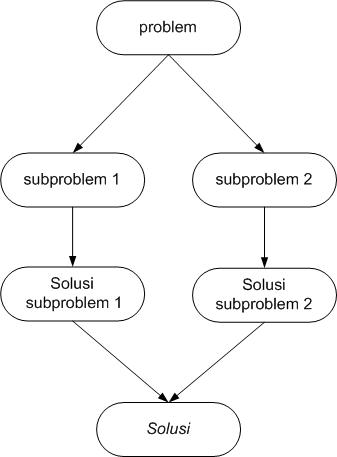
\includegraphics[scale=0.7]{fig/sunario-3/Ilustrasi.jpg}%
	\caption{Illustrasi dari Divide and Conquer}%
	\label{fig:DivideandConquerIllustration}%
\end{center}
\end{figure}

Sebagai Contoh, untuk menghitung total jumlah dari element-element dalam List, kita dapat menggunakan perulangan sederhana:



\lstset{language=Python}
\label{lst:SimpleSum}
\begin{lstlisting}[frame=single]
A = [4,1,3,5,6,7,2]
total = 0
  for i in range(0,len(A)):
    total = total + A[i]
print(total)
\end{lstlisting}

Algoritma perulangan yang digunakan pada kode di atas dapat memberikan hasil yang benar, tetapi terdapat beberapa masalah pada kode tersebut, yaitu perhitungan dilakukan secara linear, yang menghasilkan kompleksitas $O(n)$. Hal ini tentunya cukup ideal untuk ukuran list kecil, tetapi jika ukuran list menjadi besar (beberapa Milyar elemen) maka perhitungan akan menjadi sangat lambat.

Dengan menerapkan Teknik \textit{Divide and Conquer}, maka masalah penjumlahan sebelumnya dapat dibagi menjadi submasalah yang lebih kecil. Langkah pertama yang dapat dilakukan adalah menerapkan teknik rekursif untuk membagi-bagikan masalah menjadi masalah yang lebih kecil. Jika awalnya kita harus menghitung total keseluruhan list satu per satu, sekarang kita dapat melakukan perhitungan dengan memecah-mecah list terlebih dahulu:

\lstset{language=Python}
\label{lst:DivideAndConquerSum}
\begin{lstlisting}[frame=single]
def SumOfList(MyList):
  if len(MyList) <= 1:
    return MyList[0] 
	mid = len(MyList) // 2
  left = SumOfList(MyList[:mid])
  right = SumOfList(MyList[mid:])
  return left + right
	
\end{lstlisting}

Setelah membagikan list menjadi dua bagian terus menerus sampai bagian terkecilnya, penjumlahkan kedua nilai list tersebut dapat dilihat pada Figur \ref{fig:DivideAndConquerSum} berikut:

\begin{figure}[htbp]
\begin{center}
	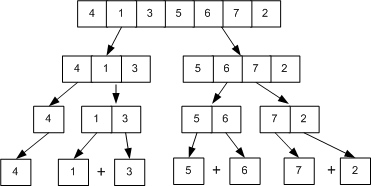
\includegraphics[scale=0.7]{fig/sunario-3/Sum.png}%
	\caption{Illustrasi Penjumlahan Divide and Conquer}%
	\label{fig:DivideAndConquerSum}%
\end{center}
\end{figure}

Algoritma \textit{Divide and Conquer}, jika diimplementasikan menggunakan library atau bahasa yang tepat akan meningkatkan efisiensi algoritma secara logaritmik. Untuk melihat kompleksitas algoritma perhatikan analisis pada fungsi SumOfList dengan teknik \textit{Divide and Conquer} berikut ini:

\lstset{language=Python}
\label{lst:DivideAndConquerSum}
\begin{lstlisting}[frame=single]
def SumOfList(MyList):
  if len(MyList) >= 1:		#cost = a 
    return MyList[0]		#cost = b 
	mid = len(MyList) // 2	#cost = c
  left = SumOfList(MyList[:mid]) #cost = f(n/2) + h
  right = SumOfList(MyList[mid:]) #cost = f(n/2) + i
  return left + right	#cost = d
	
\end{lstlisting}

yang secara matematis dapat dituliskan seperti berikut:
$$	  \mathnormal{f(n) = a+b+c+f(\frac{n}{2})+h+f(\frac{n}{2})+i+d } $$
$$	  \mathnormal{f(n) = 2f(\frac{n}{2})} $$

karena ukuran dari mid adalah panjang list $(n)$ dibagi dua. Dengan begitu, kompleksitas dari algoritma adalah:

\begin{figure}[htbp]
\begin{center}
	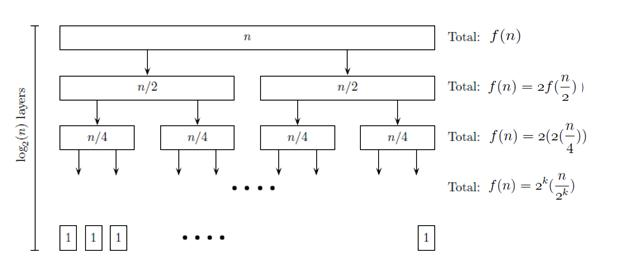
\includegraphics[scale=0.8]{fig/sunario-3/fn.jpg}%
	\caption{Illustrasi pembagian list}%
	\label{fig:PembagianList}%
\end{center}
\end{figure}

dengan syarat berhenti adalah $k \geq 1$ sehingga:

$$	  \mathnormal{ \frac{n}{2^{k}}=1} $$
$$	  \mathnormal{n=2^{k}} $$
$$	  \mathnormal{k=log_{2}n} $$

Dibandingkan dengan Algoritma penjumlahan dengan perulangan $(O(n))$, Kompleksitas dari fungsi penjumlahan dengan teknik \textit{Divide and Conquer} diatas adalah $O(log n)$.

\section{\textit{Binary Search}}
Algoritma \textit{Binary search}  merupakan  algoritma untuk melakukan pencarian pada list yang sudah mempunyai syarat bahwa list sudah terurut, baik secara menaik ataupun menurun. Algoritma \textit{Binary search} menggunakan 3 langkah dari \textit{Divide and Conquer} sebagai berikut:
\begin{enumerate}
\item \textbf{\textit{Divide}} --- Membagi $n$ elemen/bilangan menjadi dua bagian dimana masing-masing adalah $n/2$. Setiap $n$ bilangan akan terus dibagi dua menjadi dua bagian kiri dan kanan hingga data yang dicari ditemukan.
\item \textbf{\textit{Conquer}} --- Cari nilai kunci dalam  List terurut dan mengembalikan indeks di mana kunci itu ditemukan atau -1 jika tidak ditemukan dan membagi List secara rekursif.
\item \textbf{\textit{Combine}} --- Tahap ini tidak perlu dilakukan karena yang diperlukan hanya 1 element berupa data yang dicari.
\end{enumerate}

 Misalnya untuk menemukan nilai dari \textit{Val}  dalam List \textit{MyList} dengan menggunakan Algoritma \textit{Binary search}, maka ada 3 kemungkinan kondisi pada \textit{Binary search} yaitu:
\begin{enumerate}
  \item Jika nilai dari \textit{Val} di temukan pada MyList[middle], maka proses pembagian ruangan berhenti. 
  \item Jika nilai dari \textit{Val} $<$ MyList[middle], maka pencarian di batasi hanya pada bagian sebelah kiri dari List. Seluruh elemen yang berada di sebelah kanan dapat di abaikan.
  \item Jika nilai dari \textit{Val} $>$ MyList[middle], maka pencarian di batasi hanya pada bagian sebelah kanan dari List. Seluruh elemen yang berada di sebelah kiri dapat di abaikan.
  \item Jika seluruh data telah di cari namun nilai dari \textit{Val} tidak ditemukan, maka diberi nilai seperti -1.
\end{enumerate}

Sebagai Contoh, pencarian nilai 15 dari sebuah list dapat dilihat pada Figur \ref{fig:Binary Search Ilustration} berikut:

\begin{figure}[htbp]
\begin{center}
	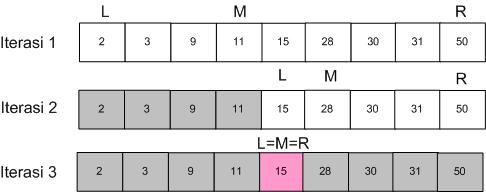
\includegraphics[scale=0.8]{fig/sunario-3/BinarySearch.jpg}%
	\caption{Illustrasi Binary Search}%
	\label{fig:Binary Search Ilustration}%
\end{center}
\end{figure}

\newpage{}
Algoritma \textit{Binary search} dapat diterapkan dengan menggunakan cara rekursif maupun nonrekursif. Untuk cara rekursif dapat diimplementasikan sebagai berikut:

\lstset{language=Python}
\label{lst:BinarySearch}
\begin{lstlisting}[frame=single]
def BinarySearch(MyList, val, left, right):
  if right < left:
    print("%d not found in list"%val)
    return -1
	
  mid = (left + right) // 2
  if MyList[mid] > val:
    return BinarySearch(MyList, val, left, mid-1)
  elif MyList[mid] < val:
    return binary_search(MyList, val, mid+1, right)
  else:
    print("%d found in index %d"%(val, mid))
  
  return mid
\end{lstlisting}

\subsection{Analisis Binary Search}
Untuk analisis metode binary search dalam menentukan kompleksitasnya, perhatikan untuk sebuah list, misalkan dengan panjang $(n) = 8$, maka :\newline
Ketika n=8, Binary Search akan mereduksi ukuran listnya menjadi 4\newline
Ketika n=4, Binary Search akan mereduksi ukuran listnya menjadi 2\newline
Ketika n=2, Binary Search akan mereduksi ukuran listnya menjadi 1\newline

Dapat dilihat bahwa binary search dipanggil sebanyak tiga kali untuk $n = 8$. Sehingga didapat $8 = 2^{3}$ atau secara general dapat dikatakan $n = 2^{k}$.  Nilai dari k dapat dinotasikan menjadi $2^{k} = n$ sehingga $k = log_2\ n$ sehingga didapatkan untuk kompleksitas dari binary search adalah  O (log n).

Misalnya jika kita memiliki list sebanyak $n$ elemen, maka kasus tersebut melakukan pembandingan list sebanyak $log\ n$. Bandingkan dengan linear search yang  melakukan pembandingan sebanyak $n$. Tentunya algoritma binary search menjadi lebih cepat. Namun jika data yang ada merupakan data yang tidak terurut maka akan jauh lebih cepat jika menggunakan linear search sehingga penggunaan binary search akan ada cost tambahan yaitu dalam mengurutkan List.

\section{\textit{Merge Sort}}
Algoritma \textit{Merge Sort} merupakan algoritma pengurutan yang mengikuti pendekatan \textit{Divide and Conquer}. Algoritma tersebut menggunakan 3 langkah dari \textit{Divide and Conquer} sebagai berikut:
\begin{enumerate}
\item \textbf{\textit{Divide}} --- Membagi $n$ elemen/bilangan menjadi dua bagian dimana masing-masing adalah $n/2$. Setiap $n$ bilangan akan terus dibagi dua sampai habis atau bilangan tinggal 1 saja.
\item \textbf{\textit{Conquer}} --- Mengurut setiap bagian secara rekursif menggunakan \textit{merge sort}. 
\item \textbf{\textit{Combine}} --- Menggabungkan dua bagian yang telah diurut untuk menghasilkan satu bagian keseluruhan yang sudah terurut.
\end{enumerate}

Figur \ref{fig:mergeSortIllustration} menggambarkan cara kerja Merge Sort terhadap 4 buah bilangan yang tak terurut. Di illustrasi tersebut \textit{List} yang memiliki 4 bilangan tak terurut dipecah-pecah sampai menjadi 1 buah bilangan atau panjang \textit{List} 1 ($A.length = 1$). Karena satu buah bilangan sudah merupakan bilangan yang terurut maka pecahan bilangan tersebut digabungkan sampai menjadi satu \textit{List} bilangan yang terurut. 

\begin{figure}[htbp]
\begin{center}
	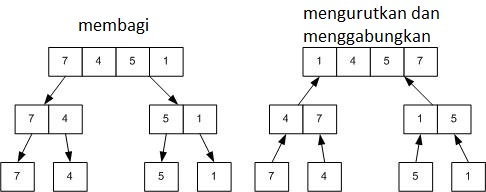
\includegraphics[scale=0.8]{fig/sunario-3/mergeSort1.jpg}%
	\caption{Illustrasi dari cara kerja merge sort}%
	\label{fig:mergeSortIllustration}%
\end{center}
\end{figure}


Algoritma \textit{merge sort} terdiri dari dua algoritma utama yaitu Algoritma (MERGE($left,right$)) dan Algoritma (MERGE-SORT($MyList$)). 

Algoritma MERGE-SORT($MyList$) ditujukan untuk membagi (\textit{divide}) sebuah \textit{List} $MyList$ menjadi dua bagian secara rekursif sampai \textit{List} tersebut tak bisa dibagi lagi (panjang \textit{List} $MyList$ adalah 1). 

\lstset{language=Python}
\label{lst:MargeSort}
\begin{lstlisting}[frame=single]
def merge_sort(A, p, r):
    if p< r:
        q = (p+r)//2
        merge_sort(A, p, q)
        merge_sort(A, q+1, r)
        merge(A,p,q,r)
\end{lstlisting}

Algoritma MERGE($left,right$) ditujukan untuk menggabungkan (\textit{combine}) kumpulan \textit{List} yang sudah diurut (memiliki panjang 1) menjadi sebuah \textit{List} baru yang sudah terurut.

\lstset{language=Python}
\label{lst:Marge}
\begin{lstlisting}[frame=single]
def merge(A,p,q,r):
    n1 = q-p+1
    n2 = r-q
    L =[]
    R =[]
    for i in range(0,n1):
        L.append(A[p+i])
    for j in range(0,n2):
        R.append(A[q+j+1])
    L.append(float("inf"))
    R.append(float("inf"))
    i = 0
    j =0
    for k in range(p, r+1):
        if L[i] <= R[j]:
            A[k] = L[i]
            i = i + 1
        else:
            A[k] = R[j]
            j = j + 1

\end{lstlisting}

Perlu diketahui di algoritma \textit{merge sort} tidak diperlukan fungsi khusus untuk \textit{Conquer} dikarenakan \textit{List} yang memiliki panjang 1 secara otomatis sudah terurut.

\newpage{}
\subsection{Analisis Merge Sort}
Seberapa efisienkah \textit{merge sort}? Berikut analisis dari kompleksitas \textit{merge sort}.

\lstset{language=Python}
\label{lst:MargeSort}
\begin{lstlisting}[frame=single]
def merge_sort(A, p, r):
    if p< r:                    #cost = a
        q = (p+r)//2            #cost = b
        merge_sort(A, p, q)     #cost = f(n/2) + h
        merge_sort(A, q+1, r)   #cost = f(n/2) + i
        merge(A,p,q,r)          #cost = g.n + j
\end{lstlisting}

yang secara matematis dapat dituliskan seperti berikut:
$$	  \mathnormal{f(n) = a+b+f(\frac{n}{2})+h+f(\frac{n}{2})+i+g.n+j } $$
$$	  \mathnormal{f(n) = 2f(\frac{n}{2})+a.n + b} $$

dengan syarat $n > 1$, maka:
$$	  \mathnormal{f(n) = 2f(\frac{n}{2})+a.n } $$
$$	  \mathnormal{f(n) = 2(2f(\frac{n}{4})+a.\frac{n}{2} )} + a.n $$
$$	  \mathnormal{f(n) = 4f(\frac{n}{4})+2a.n } $$
$$	  \mathnormal{f(n) = 4(2f(\frac{n}{8})+a.\frac{n}{4} )}+2a.n $$
$$	  \mathnormal{f(n) = 8f(\frac{n}{8})+3a.n } $$
$$	  \mathnormal{f(n) = 16f(\frac{n}{16})+4a.n } $$
$$	  \mathnormal{f(n) = 2^{k}f(\frac{n}{2^{k}})+k.a.n } $$

untuk $ \mathnormal{f(n) = (\frac{n}{2^{k}})} $ :

$$ \mathnormal{\frac{n}{2^{k}}} $$
$$ \mathnormal{2^{k}=n} $$
$$ \mathnormal{k=log_{2}n} $$

sehingga :

$$	  \mathnormal{f(n) = 2^{log_{2}n}f(1)+log_{2}n.a.n } $$

$$	  \mathnormal{f(n) = a.n\ log\ n = O(n\ log\ n)} $$
 
\section{\textit{Quick Sort}}

\textit{Quick sort} seperti \textit{merge sort} juga menggunakan pendekatan \textit{Divide and Conquer}. Tiga langkah yang dimiliki \textit{quick sort} ialah:
\begin{enumerate}
	\item \textit{Divide} --- Mempartisi (menyusun) \textit{List} $MyList[p..r]$ menjadi dua \textit{list} yang berukuran lebih kecil yaitu $MyList[l..q-1]$ dan $MyList[q+1..r]$ sehingga setiap elemen dari $MyList[l..q-1]$ lebih kecil atau sama dengan $A[q]$ yang mana akan lebih kecil atau sama dari setiap elemen $A[q+1..r]$. Indeks $q$ dihitung melalui fungsi partisi.
	\item \textit{Conquer} --- Urut dua \textit{list} $A[p..q-1]$ dan $A[q+1..r]$ secara rekursif.
	\item \textit{Combine} --- Tahap ini tidak perlu dilakukan karena sudah tergabung secara otomatis.
\end{enumerate}

Teknik \textit{Quick sort} berbeda teknik \textit{merge sort} dimana \textit{merge sort} membagi elemen-elemen dalam list berdasarkan posisi, \textit{quick sort} membagi elemen-elemen dalam List tersebut berdasrkan nilai. Secara spesifik, \textit{quick sort} mengatur kembali setiap elemen yang ada dalam list berdasarkan \emph{partisinya}. Sebuah variasi dari algoritma \textit{quick sort} adalah algoritma \textit{randomized-quick sort} dimana di algoritma tersebut memilih \textit{partisi} secara acak (\textit{random}). Hal tersebut dilakukan dengan harapan pemotongan rangkaian (\textit{partition}) lebih terdistribusi secara merata.

\newpage{}
Adapun ilustrasi dari cara kerja dari \textit{quick sort} dapat dilihat pada Figur \ref{fig:Quick Sort Ilustration} berikut:

\begin{figure}[htbp]
\begin{center}
	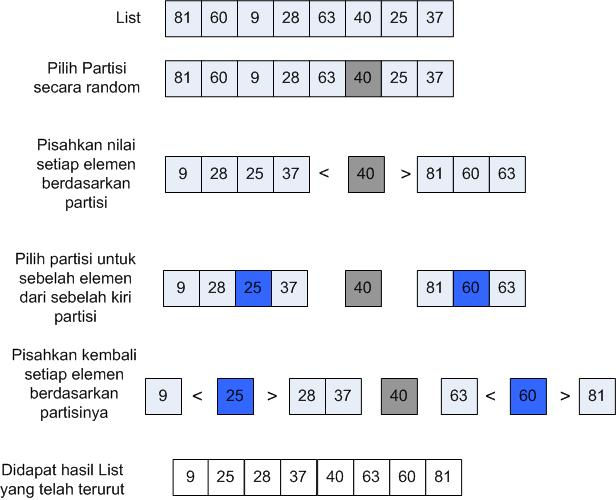
\includegraphics[scale=0.8]{fig/sunario-3/QuickSort.jpg}%
	\caption{Ilustrasi Quick Sort}%
	\label{fig:Quick Sort Ilustration}%
\end{center}
\end{figure}

Kerugian dari versi sederhana diatas adalah membutuhkan ruang simpan yang lebih besar, yang sama buruknya seperti merge sort. Memory tambahan yang dibutuhkan dapat juga secara radikal berpengaruh pada kecepatan dan performa cache pada implementasi praktiknya. Terdapat juga versi yang lebih rumit yang menggunakan algoritma partisi \textit{in-place}. Ilustrasi dari algoritma \textit{quick sort} dengan partisi \textit{in-place}. Algoritma partisi \textit{in-place} digunakan untuk memisahkan bagian dari list antara index kiri dan kanan, dengan memindahkan seluruh elemen kurang dari MyList[pivotIndex] sebelum pivot, dan elemen yang sama atau lebih besar darinya. Dalam prosesnya, algoritma ini juga mencari posisi akhir untuk elemen pivot kembali. 


Adapun ilustrasi dari cara kerja dari \textit{quick sort} dengan partisi \textit{in-place} dapat dilihat pada Figur \ref{fig:Quick Sort Ilustration 2} berikut:

\begin{figure}[htbp]
\begin{center}
	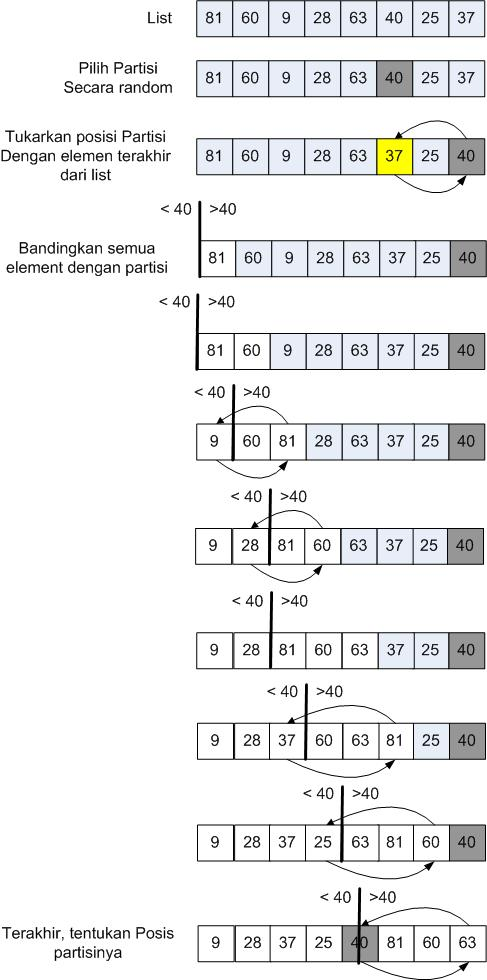
\includegraphics[scale=0.5]{fig/sunario-3/QuickSort2.jpg}%
	\caption{Ilustrasi Quick Sort In-Place}%
	\label{fig:Quick Sort Ilustration 2}%
\end{center}
\end{figure}

\newpage{}
Dalam Python Algoritma \textit{quick sort} dapat diterapkan sebagai berikut:
\lstset{language=Python}
\label{lst:QuickSort}
\begin{lstlisting}[frame=single]
def quickSort(A, p, r):
 if p < r:
   q = partition(A, p, r)
   quickSort(A, p, q-1)
   quickSort(A, q+1, r)
\end{lstlisting}

\lstset{language=Python}
\label{lst:Partition}
\begin{lstlisting}[frame=single]
def partition(A,p,r):
    x = A[r]
    i = p-1
    for j in range(p,r):
        if(A[j] <= x):
            i = i + 1
            A[i],A[j] = A[j],A[i]
    A[i+1],A[r] = A[r],A[i+1]
    return i+1
\end{lstlisting}

\subsection{Analisis Quick Sort}
Kompleksitas dari \textit{quick sort} tergantung pada  seimbang atau tidak seimbang pembagian partisi pada list yang akan diurutkan. Sebuah partisi yang  baik membagi list menjadi dua list dengan ukuran sama, sedangkan partisi yang buruk membagi list menjadi dua list dengan ukuran yang sangat berbeda. Partisi terburuk menempatkan hanya satu elemen dalam satu list dan semua elemen lainnya dalam list lain. 

Untuk menganalisi kompleksitas dari \textit{quick sort}, terlebih dahulu, perlu diperhitungkan kompleksitas dari algoritma partisi yang digunakan karena algoritma partisi yang digunakan bukan pernyataan sederhana.

\lstset{language=Python}
\label{lst:Partition}
\begin{lstlisting}[frame=single]
def partition(A,p,r):
    x = A[r]                       #cost a
    i = p-1                        #cost b
    for j in range(p,r):
        if(A[j] <= x):
            i = i + 1
            A[i],A[j] = A[j],A[i]  #cost j.n+c
    A[i+1],A[r] = A[r],A[i+1]      #cost d
    return i+1                     #cost e
\end{lstlisting}

Didalam algoritma partisi yang digunakan, terdapat sebuah loop for yang diikuti oleh statement sederhana lainnya. Statement sederhana tersebut dapat diberikan $f(n)= a+b+d+e$, kecuali yang berada di dalam statement for, dimana nilai $f(n) = j.n+c/O(n)$. Sehingga didapatkan kompleksitas untuk algoritma partisi diatas adalah :

$$ \mathnormal{f(n) = a+b+j.n+c+d+e} $$
$$ \mathnormal{f(n) = j.n} $$

Setelah mendapatkan nilai kompleksitas dari algoritma partisiya, maka dapat dihitung kompleksitas untuk algoritma \textit{quick sort} .

\lstset{language=Python}
\label{lst:QuickSort}
\begin{lstlisting}[frame=single]
def quickSort(A, p, r):
 if p < r:                #cost a
   q = partition(A, p, r) #cost j.n
   quickSort(A, p, q-1)   #cost f(n/2) + b
   quickSort(A, q+1, r)   #cost f(n/2) + c
\end{lstlisting}

yang secara matematis dapat dituliskan seperti berikut:
$$	  \mathnormal{f(n) = a+j.n+f(\frac{n}{2})+b+f(\frac{n}{2})+c } $$
$$	  \mathnormal{f(n) = 2f(\frac{n}{2})+j.n } $$

dengan syarat $n > 1$, maka:
$$	  \mathnormal{f(n) = 2f(\frac{n}{2})+j.n } $$
$$	  \mathnormal{f(n) = 2(2f(\frac{n}{4})+j.\frac{n}{2} )} + j.n $$
$$	  \mathnormal{f(n) = 4f(\frac{n}{4})+2j.n } $$
$$	  \mathnormal{f(n) = 4(2f(\frac{n}{8})+j.\frac{n}{4} )}+2j.n $$
$$	  \mathnormal{f(n) = 8f(\frac{n}{8})+3j.n } $$
$$	  \mathnormal{f(n) = 16f(\frac{n}{16})+4j.n } $$
$$	  \mathnormal{f(n) = 2^{k}f(\frac{n}{2^{k}})+k.j.n } $$

untuk $ \mathnormal{f(n) = (\frac{n}{2^{k}})} $ :

$$ \mathnormal{\frac{n}{2^{k}}=1} $$
$$ \mathnormal{2^{k}=n} $$
$$ \mathnormal{k=log_{2}n} $$

sehingga :

$$	  \mathnormal{f(n) = 2^{log_{2}n}f(1)+log_{2}n.j.n } $$

$$	  \mathnormal{f(n) = j.n\ log\ n = O(n\ log\ n)} $$

Untuk Worse Case dari \textit{quick sort} , jika partisinya dibagi tidak sama rata atau hanya satu elemen dalam satu list dan semua elemen lainnya dalam list lain seperti Figur \ref{fig:WorseCaseQuickSort}, maka kompleksitasnya adalah:

$$	  \mathnormal{f(n) = f(n-1)+j.n} $$
$$	  \mathnormal{f(n) = f(n-2)+j(n-1)+(j.n)} $$
$$	  \mathnormal{f(n) = f(n-2)+2(j.n)} $$
$$	  \mathnormal{f(n) = f(n-3)+j(n-2))+2(j.n)} $$
$$	  \mathnormal{f(n) = f(n-3)+3(j.n)} $$
$$	  \mathnormal{f(n) = f(n-4)+4(j.n)} $$
$$	  \mathnormal{f(n) = f(n-k)+k(j.n)} $$

untuk $ \mathnormal{f(n) = k.n  }$:
$$ \mathnormal{ k.n = 1  }$$
$$ \mathnormal{ k = n }$$

sehingga :

$$ \mathnormal{f(n) = f(1) + n.j.n} $$
$$ \mathnormal{f(n) = j.n^{2} = O(n^{2})} $$
		

\begin{figure}[htbp]
\begin{center}
	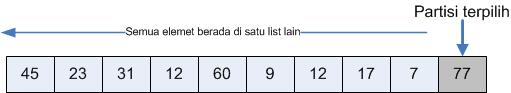
\includegraphics[scale=0.5]{fig/sunario-3/QuickSort3.jpg}%
	\caption{Quick Sort Worse Case}%
	\label{fig:WorseCaseQuickSort}%
\end{center}
\end{figure}


Jika partisi seimbang, maka kompleksitas dari  \textit{quick sort} berjalan secepat merge sort $O(n\ log\ n)$. Di sisi lain, jika partisi tidak seimbang, \textit{quick sort} berjalan lambat seperti insertion sort $O(n^{2})$.

\end{document}
